%%
%% This is file `sample-sigconf.tex',
%% generated with the docstrip utility.
%%
%% The original source files were:
%%
%% samples.dtx  (with options: `sigconf')
%% 
%% IMPORTANT NOTICE:
%% 
%% For the copyright see the source file.
%% 
%% Any modified versions of this file must be renamed
%% with new filenames distinct from sample-sigconf.tex.
%% 
%% For distribution of the original source see the terms
%% for copying and modification in the file samples.dtx.
%% 
%% This generated file may be distributed as long as the
%% original source files, as listed above, are part of the
%% same distribution. (The sources need not necessarily be
%% in the same archive or directory.)
%%
%% The first command in your LaTeX source must be the \documentclass command.

\documentclass[sigconf]{acmart}
% \documentclass[sigconf,review]{acmart}
% \documentclass[sigconf,review,anonymous]{acmart}
\acmSubmissionID{pap242}

\usepackage[utf8x]{inputenc} % allow utf-8 input
\usepackage[T1]{fontenc}    % use 8-bit T1 fonts
\usepackage{booktabs}       % professional-quality tables
\usepackage{textgreek}
\usepackage[scaled=0.85]{DejaVuSansMono}

% \usepackage{todonotes}
\usepackage[mode=buildnew]{standalone}
\usepackage{minted}
\usepackage{listings}
\usepackage{bm}
\usepackage[usenames,dvipsnames]{pstricks}
\usepackage{import}

\usepackage{subcaption}
\newcommand{\REAL}{\mathbb{R}}
\newcommand{\bigo}[1]{\mathcal{O}\left( #1 \right)}

% various reference macros
\newcommand{\refalg}[1]{Algorithm~\ref{#1}}
\newcommand{\refsec}[1]{Section~\ref{#1}}
\newcommand{\reffig}[1]{Figure~\ref{#1}}
\newcommand{\refsubfig}[1]{Figure~\subref{#1}}
\newcommand{\reftab}[1]{Table~\ref{#1}}
\newcommand{\refeqn}[1]{(\ref{#1})}
\newcommand{\reflst}[1]{Listing~(\ref{#1})}
\newcommand{\defn}[1]{\textbf{\textit{#1}}}
\newmintinline[txtcode]{cpp}{
  fontsize=\small\tt,
  escapeinside=||,
}
\newminted[code]{cpp}{
  fontsize=\small,
  escapeinside=||,
}

\usepackage{marvosym}

%%
%% \BibTeX command to typeset BibTeX logo in the docs
\AtBeginDocument{%
  \providecommand\BibTeX{{%
    \normalfont B\kern-0.5em{\scshape i\kern-0.25em b}\kern-0.8em\TeX}}}

%% Rights management information.  This information is sent to you
%% when you complete the rights form.  These commands have SAMPLE
%% values in them; it is your responsibility as an author to replace
%% the commands and values with those provided to you when you
%% complete the rights form.
\copyrightyear{2021}
\acmYear{2021}
\setcopyright{licensedusgovmixed}

\acmConference[SC '21]{The International Conference for High Performance Computing, Networking, Storage and Analysis}{November 14-19, 2021}{St. Louis, MO, USA}
\acmBooktitle{The International Conference for High Performance Computing, Networking, Storage and Analysis (SC '21), November 14-19, 2021, St. Louis, MO, USA}
\acmPrice{15.00}
\acmDOI{10.1145/3458817.3476165}
\acmISBN{978-1-4503-8442-1/21/11}


\newcommand{\subheading}[1]{{\textbf{\textit{#1}}\\}}
\newcommand{\wmnote}[1]{{\color{blue} Billy: #1}}
\newcommand{\vcnote}[1]{{\color{brown} Valentin: #1}}
\newcommand{\define}[1]{\textbf{\emph{#1}}}
\newcommand{\grad}{\hspace*{-.5mm}{\fontsize{8}{8}\selectfont∇}\hspace*{0mm}}

% \newcommand{\change}[1]{{\color{blue} #1}}
\newcommand{\change}[1]{{#1}}

%% These commands are for a PROCEEDINGS abstract or paper.
% \overfullrule=1mm
%%
%% Submission ID.
%% Use this when submitting an article to a sponsored event. You'll
%% receive a unique submission ID from the organizers
%% of the event, and this ID should be used as the parameter to this command.
%%\acmSubmissionID{123-A56-BU3}

%%
%% The majority of ACM publications use numbered citations and
%% references.  The command \citestyle{authoryear} switches to the
%% "author year" style.
%%
%% If you are preparing content for an event
%% sponsored by ACM SIGGRAPH, you must use the "author year" style of
%% citations and references.
%% Uncommenting
%% the next command will enable that style.
%%\citestyle{acmauthoryear}

%%
%% end of the preamble, start of the body of the document source.
\begin{document}

%%
%% The "title" command has an optional parameter,
%% allowing the author to define a "short title" to be used in page headers.
\title{Reverse-Mode Automatic Differentiation and Optimization of GPU Kernels via Enzyme}
% $\frac{\partial \text{Enzyme}}{\partial \text{GPU}}$
% Enzyme++
% Enzyme<<<CUDA>>>
% \nabla CUDA
%%
%% The "author" command and its associated commands are used to define
%% the authors and their affiliations.
%% Of note is the shared affiliation of the first two authors, and the
%% "authornote" and "authornotemark" commands
%% used to denote shared contribution to the research.
\author{William S. Moses$^*$,\hspace{1em} Valentin Churavy $^*$,\hspace{1em} Ludger Paehler$^{\mathsection}$,\hspace{1em} Jan Hückelheim $^\dagger$,\\ Sri Hari Krishna Narayanan  $^\dagger$,\hspace{1em} Michel Schanen  $^\dagger$,\hspace{1em} Johannes Doerfert$^\dagger$}
\email{{wmoses,vchuravy}@mit.edu, 
ludger.paehler@tum.de,
{jhuckelheim,snarayan,mschanen,jdoerfert}@anl.gov}
\affiliation{%
  \institution{MIT CSAIL $^*$,\hspace{1em} Technical University of Munich $^{\mathsection}$,\hspace{1em} Argonne National Laboratory$^\dagger$}\country{}
}

%%
%% By default, the full list of authors will be used in the page
%% headers. Often, this list is too long, and will overlap
%% other information printed in the page headers. This command allows
%% the author to define a more concise list
%% of authors' names for this purpose.
\renewcommand{\shortauthors}{Moses, Churavy, Paehler, Hückelheim, Narayanan, Schanen, and Doerfert}

%%
%% The abstract is a short summary of the work to be presented in the
%% article.
\begin{abstract}
\if 1
Derivatives are key to algorithms in scientific computing and machine learning such as optimization, uncertainty quantification, and stability analysis. Enzyme is a LLVM compiler plugin for reverse-mode automatic differentiation (AD) and thus generates fast gradients of programs in a variety of languages, including C/C++, Fortran, Julia, and Rust. Our paper presents a combination of novel techniques that make Enzyme the first automatic reverse-mode AD tool to generate gradients of GPU kernels. As Enzyme differentiates within a general-purpose compiler, we are able to introduce novel GPU and AD-specific optimizations. We differentiate five GPU-based HPC applications, executed on NVIDIA and AMD GPUs. All benchmarks run within an order of magnitude of the original program's runtime. Without GPU and AD-specific optimizations, gradients of GPU kernels either fail to run from a lack of resources or have infeasible overhead. We show that increasing the problem size does not substantially impact the overhead from differentiation.
\else
  %In this paper, we present the first automatic differentiation tool that can generate gradients of CUDA kernels.

  Computing derivatives is key to many algorithms in scientific computing and machine learning such as optimization, uncertainty quantification, and stability analysis. %
  %
  %Reverse-mode automatic differentiation (AD) is a technique for simultaneously computing the derivative of all input variables (gradient). For multi-parameter computations reverse mode can be asymptotically faster than other techniques.
  %
  Enzyme is a LLVM \change{compiler plugin} that performs reverse-mode automatic differentiation (AD) and thus generates high performance gradients of programs in languages including C/C++, Fortran, Julia, and Rust. Prior to this work, Enzyme and other AD tools were not capable of generating gradients of GPU kernels. 
%
%   \change{ Reverse-mode AD of GPU kernels hasn't been explored historically due to performance and correctness challenges from the GPU's inherent parallel nature, complex performance characteristics, and the need to preserve data dependencies.}
%
  Our paper presents a combination of novel techniques that make Enzyme the first fully automatic reverse-mode AD tool to generate gradients of GPU kernels.
  \change{Since unlike other tools Enzyme performs automatic differentiation within a general-purpose compiler, we are able to introduce several novel GPU and AD-specific optimizations. }
  To show the generality and efficiency of our approach, we \change{compute gradients }of five GPU-based HPC applications, executed on NVIDIA and AMD GPUs. \change{ All benchmarks run within an order of magnitude of the original program's execution time. Without GPU and AD-specific optimizations, gradients of GPU kernels either fail to run from a lack of resources or have infeasible overhead.
  %Through an explicit ablation analysis, we demonstrate that without GPU and AD-specific optimizations, gradients of GPU kernels may have runtimes which are several orders of magnitude slower than the original code, if they even run at all.
  %In contrast, by enabling optimizations, the gradient kernels have similar runtimes to the original program
  } \change{Finally, we demonstrate that increasing the problem size by either increasing the number of threads or increasing the work per thread, does not substantially impact the overhead from differentiation.}
%  \change{ We demonstrate that without being able to apply GPU and AD-specific optimizations, the generated gradients of GPU kernels may take several orders of magnitude longer to evaluate. without novel the GPU-specific and}
  % AD-specific optimizations in our paper, gradients of GPU kernels 
  % Through the use of \change{novel} GPU-specific and AD-specific compiler optimizations we \change{generate gradients of GPU kernels with similar performance to the original program.} reverse mode AD for GPU kernels feasible   and as efficient as $1.7\times$ the time a forward pass takes to run the LULESH~\cite{LULESH2:changes} benchmark. 
  
  

  %---------- end of abstract
\fi
\end{abstract}

%   Computing derivatives is key to optimization, uncertainty quantification, stability analysis, and related methods in scientific computing and machine learning.
%%
%% The code below is generated by the tool at http://dl.acm.org/ccs.cfm.
%% Please copy and paste the code instead of the example below.
%%
\begin{CCSXML}
<ccs2012>
<concept>
<concept_id>10002950.10003714.10003715.10003748</concept_id>
<concept_desc>Mathematics of computing~Automatic differentiation</concept_desc>
<concept_significance>500</concept_significance>
</concept>
<concept>
<concept_id>10011007.10011006.10011041.10011047</concept_id>
<concept_desc>Software and its engineering~Source code generation</concept_desc>
<concept_significance>500</concept_significance>
</concept>
<concept>
<concept_id>10003752.10003753.10003761.10003762</concept_id>
<concept_desc>Theory of computation~Parallel computing models</concept_desc>
<concept_significance>300</concept_significance>
</concept>
<concept>
<concept_id>10003752.10003809.10010170.10010171</concept_id>
<concept_desc>Theory of computation~Shared memory algorithms</concept_desc>
<concept_significance>300</concept_significance>
</concept>
<concept>
<concept_id>10010147.10010257</concept_id>
<concept_desc>Computing methodologies~Machine learning</concept_desc>
<concept_significance>300</concept_significance>
</concept>
</ccs2012>
\end{CCSXML}

\ccsdesc[500]{Mathematics of computing~Automatic differentiation}
\ccsdesc[500]{Software and its engineering~Source code generation}
\ccsdesc[300]{Theory of computation~Parallel computing models}
\ccsdesc[300]{Theory of computation~Shared memory algorithms}
\ccsdesc[300]{Computing methodologies~Machine learning}


%%
%% Keywords. The author(s) should pick words that accurately describe
%% the work being presented. Separate the keywords with commas.
\keywords{Automatic Differentiation, AD, CUDA, ROCm, GPU, LLVM, HPC}


%%
%% This command processes the author and affiliation and title
%% information and builds the first part of the formatted document.
\maketitle

\section{Introduction}
\label{sec:intro}

Automatic differentiation (AD) provides an accurate way of computing derivatives of mathematical functions that are implemented in computer programs. \emph{Gradients} (or \emph{adjoints}), a special case of derivatives for functions with one output and many inputs, have applications in optimization \cite{duchi2011adaptive}, uncertainty quantification \cite{ghanem2017handbook}, inverse design, stability analysis,%GAIL - nor refs?
and machine learning \cite{maclaurin2015gradient}. Reverse-mode AD  has been the tool of choice to compute these gradients for large applications with many input parameters.

% Automatic differentiation (AD) provides an accurate way of computing derivatives of multivariate vector function implementations $\bm{y} = f(\bm{x}),\, \REAL^n \mapsto \REAL^m$ with input $\bm{x}$ and output $\bm{y}$. With a variety of approaches for calculating these derivatives automatically, ranging from source transformation to operator overloading, this paper focuses on a compiler integrated solution through LLVM. There are two modes of differentiation. The tangent-mode generates the implementation of the Jacobian vector product $\dot{\bm{y}} = \nabla f(\bm{x}) \cdot \dot{\bm{x}}$, whereas reverse-mode AD computes the transposed Jacobian vector product $\bar{\bm{x}} = \bar{\bm{y}} \cdot \nabla f(\bm{x})^T$, with $\dot{}$ and $\bar{}$ denoting directional derivatives and adjoints, respectively.  Computing \emph{gradients} in reverse mode, a special case of derivatives with one output $m=1$ and many inputs $n$, is of particular usefulness for applications in optimization, uncertainty quantification, inverse design, stability analysis, and machine learning, as the resulting gradient implementation has a complexity of $\bigo{cost(f)}$, independent of $n$.

As the research community has been continuously pushing the boundary of the size of problems they want to solve, large-scale applications have had to leverage the latest in high-performance computing including distributed computation, parallelism, and accelerators. % Many  machine learning and scientific computing applications rely on kernels that are highly optimized for graphics processing units (GPUs). 
For many machine learning and scientific computing applications, this means relying on kernels that are highly optimized for graphics processing units (GPUs). 
% For many machine learning and scientific computing applications, this means optimizing your code for graphics processing units (GPUs).
%(for NVIDIA GPU's) or ROCm (for AMD GPU's)

\begin{figure}
    \centering
%\textbf{(a)}\\
\begin{minipage}[T]{0.95\linewidth}
\begin{code}
|\;|
void init(double* ar, int N, double val) {
  parallel_for(int i=0; i<N ; i++)
    // Concurrent reads of val
    ar[i] = val;
}

double gradient_init(double* ar, double* d_ar,
                     int N, double val) {
  double d_val = 0.0;
  parallel_for(int i=0; i<N ; i++)
    ar[i] = val;
  parallel_for(int i=0; i<N ; i++) {
    // Concurrent writes to d_val
    d_val += d_ar[i];                  |\Large\textcolor{red}{{\Lightning{}} race {{}\Lightning{}}}|
    d_ar[i] = 0.0;
  }
  return d_val;
}
|\;|
\end{code}
\end{minipage}
\vspace*{-3mm}
    \caption{
    A parallel initialize function (top) with a naive reverse mode AD gradient function (bottom) that does not take the parallelism into account.
    Consequently, the concurrent read of the variable \txtcode{val} causes a race in the reverse-mode gradient computation.
%    Without taking into consideration parallelism, a benign read race in the function \texttt{init} (a) leads to a write race in the reverse pass of the corresponding gradient computation \texttt{gradient\_init} (b).
}
    \label{fig:benign_read}
\end{figure}

While  considerable effort has  been expended to compute gradients of MPI and OpenMP programs (see Sec~\ref{sec:related} for related work), no AD tool has been presented to date that can compute gradients of CUDA or ROCm (AMD) kernels. The cause rests with both the GPU's parallelism and its complex performance characteristics. The biggest issue for both performance and correctness is due to the implied computational flow reversal of reverse-mode AD; every read becomes a write in the adjoint computation and vice versa. Consider the program \change{at the top of} Figure \ref{fig:benign_read}. It contains a simple parallel for loop that reads from the same variable \texttt{val} in all threads and sets each index of the output array \texttt{ar} to that value. Since all threads read the same value, there is a \textit{concurrent read access} on \texttt{val}, which does not impact the final result. Computing the gradient function of this program (i.e. the derivative of the input \texttt{val}), one must accumulate all of the partial derivatives of \texttt{val} generated by uses in the outputs. Such an action unfortunately leads to a \textit{write race} on the gradient \texttt{d\_val}, which may be updated by multiple threads at the same time. Special care must be taken to avoid undefined behavior and ensure the correctness of the gradient computation while preserving as much of its parallelism as possible.

GPUs often have relatively small amounts of memory per thread. Moreover, the memory of GPUs commonly has complex performance characteristics, with global memory being slow but large, shared memory being fast but small, 
and the use of certain types of memory preventing the simultaneous use of large thread counts. Potential remedies involve either sacrificing generality, by rewriting HPC applications in a differentiable domain-specific language (DSL), or resorting  to  approaches such as numerical differentiation. 

% require  , which is by nature more amendable to single instruction multiple data (SIMD) architectures like GPUs, because each component of the gradient can be independently computed. Despite this advantage, forward mode and vector forward mode both must evaluate the function a linear of a complexity of $\bigo{n\cdot cost(f)}$, where $n$ is the dimension of the gradient. Although reverse-mode automatic differentiation has a higher constant factor in its complexity of $\bigo{cost(f)}$, the gradient (derivative of all input parameters) amounts to a single function evaluation. This makes forward mode AD or finite differences intractable for programs with a large number of parameters such as neural networks, potential functions, and numerical simulations. 

To leverage the potential performance benefits of reverse-mode AD without sacrificing generality, one requires a tool that is  capable of both  handling the complex performance characteristics of GPU architectures and generating code that maintains the correctness of the gradient without sacrificing the inherent parallelism of the original program. 
Unlike many other tools, Enzyme\footnote{https://enzyme.mit.edu}~\cite{enzymeNeurips} performs AD alongside the traditional optimization pipeline by performing differentiation within the LLVM compiler~\cite{LLVM}. Thus,  we  can leverage existing code transformation infrastructure to build the requisite analyses and transformations for maintaining the correctness and performance of the corresponding gradient kernel. Furthermore, LLVM provides frontends for most commonly used languages including C/C++, Fortran, Julia, Rust, Swift, and TensorFlow and backends for different hardware architectures including CPU, NVIDIA GPUs \cite{rhodin2010ptx,holewinski2011ptx, gpucc}, and AMD GPUs, allowing us to build reverse-mode AD for multiple languages and architectures.

%\vfill\break
Overall, our paper makes the following contributions:
\begin{itemize}
    \item An algorithm for correctly generating gradients of GPU kernels and a corresponding proof sketch of correctness
    \item An extension to the Enzyme AD engine for LLVM that can generate gradients for GPU kernels written in either CUDA (NVIDIA) or ROCm (AMD)
    \item A collection of optimization passes for Enzyme/LLVM that allow generated GPU gradients to run efficiently on modern hardware
    \item A study demonstrating, for the first time, the feasibility of reverse-mode automatic differentiation of GPU kernels through the use of GPU and AD-specific optimizations (cach\-ing and re\-computation).
\end{itemize}

% Rewritten into the above
% While there are methods for obtaining Jacobians, Hessians and higher-order derivatives for arbitrarily-shaped functions, we focus in this work on gradient or adjoint computations which ask for the derivative of many inputs with respect a few outputs. This is an important special case, since many functions of practical interest have only one output  -- often a cost function, misfit, or similar -- and a large number of inputs such as design parameters, neural network weights, initial state variables, etc. As a result, gradient computations form the core of algorithms such as neural networks training, design optimization, and potential-based scientific simulation. The \emph{reverse mode} of AD is able to compute the derivative of all input gradient with a constant factor run time overhead. This is in contrast to simpler approaches like finite differences, also known as numerical differentiation, and forward-mode AD which require at least one perturbed function evaluation per input and thus have a run time overhead that scales linearly with the input size.

% Many applications for which gradients are required have been optimized for performance and use parallel hardware through MPI, OpenMP, CUDA, and ROCm (AMD). Consequently, it is desirable to have AD approaches that can handle parallel input programs. While there has been considerable effort in the past to compute gradients of MPI and OpenMP programs~\cite{5161165}, no AD tool has been presented to date that can compute gradients of CUDA or ROCm (AMD) kernels. Generally, gradient computation of parallel programs is known to be a hard problem [TODO cite], since reverse mode AD introduces additional data dependencies and potential race conditions. Efficient reverse mode AD of GPU kernels is even more challenging due to the severely constrained memory size and the need for non-trivial optimizations that do not easily carry over to the gradient computation.

% In this work, we present an extension to the freely available, open source Enzyme AD tool~\footnote{https://enzyme.mit.edu} that enables gradient computation of CUDA (NVIDIA) and ROCm (AMD) kernels through reverse mode AD. Enzyme is a plugin to the LLVM compiler that previously supported sequential programs written, for example, in C/C++, Julia, or Rust. Our extension combines existing LLVM optimizations with several new analyses and code transformations to efficiently compute gradients, which requires to resolve potential data race issues, differentiate parallel control (syncthreads), CUDA intrinsics (e.g. threadIdx.x), and handle shared memory. Our extension is now part of the latest Enzyme version and enabled by default.

% Eval description moved to results

% if we need space I'd be ok cutting the traditional systems paper layout of sections -wm

% The rest of the paper is structured as follows.
% We briefly summarize related work
% in Section~\ref{sec:related}.
% In Section~\ref{sec:method},
% we explain our overall methodology
% and its implementation.
% Section~\ref{sec:opt} describes the code analysis and optimization approaches that we use for better performance. We evaluate the performance of our approach in Section~\ref{sec:eval}
% and conclude with final remarks in Section~\ref{sec:conclusion}.

%\begin{itemize}
%    \item By extending Enzyme, to make it the first AD tool to reverse diff CUDA kernels
%        \item Race resolution in reverse
%        \item Sync <--
%        \item Misc CUDA [threadIdx, shared mem, etc]
%        \item Optimize to fit in GPU [mem] <--
%
%    \item Parallel Enzyme (GPU) is based on LLVM (C++ + Julia)
%
%    \item Gradients are useful in science and ML
%        \item Permeating new hybrid constructions in the sciences such as diff programming, neural PDEs etc.
%        
%    \item A few words about existing AD approaches
%        \item Fwd diff
%        \item DSL
%        \item set of known functions
%        
%    \item x Y speedups in our test cases, name test cases
%\end{itemize}
%
%Sentence fragments from the abstract:
%\begin{itemize}
%    \item We present an extension to Enzyme capable of modeling and differentiating parallel, and specifically GPU programs.
%    \item By working at the compiler level we are able to create a single infrastructure capable of differentiating multiple types of parallelism.
%    \item This involves preventing races in the reverse pass.
%    \item We further demonstrate the need to combine traditional optimizations with differentiation by both an ablation analysis of applying existing LLVM optimizations, as well as new AD-aware optimizations.
%    \item We present an extension to Enzyme capable of modeling and differentiating parallel, and specifically GPU programs.
%    \item In this paper, we present an extended version of Enzyme that is the first automatic differentiation tool that can generate gradients (reverse mode AD) of CUDA kernels.
%\end{itemize}
%
%Automatic differentiation (AD) is key to training neural networks, bayesian inference, and scientific computing. Applying these techniques requires rewriting code in a specific machine learning framework or manually providing derivatives. This talk presents Enzyme, a high performance automatic differentiation (AD) compiler plugin for the LLVM compiler capable of synthesizing gradients of programs expressed in the LLVM intermediate representation (IR). Enzyme differentiates programs in any language whose compiler targets LLVM including C/C++, Fortran, Julia, Rust, Swift, etc., thereby providing native AD capabilities in these languages with state of the art performance. Unlike traditional tools, Enzyme performs AD on optimized IR. On a machine-learning benchmark suite, AD on optimized IR achieves a geometric mean speedup of 4.5x over AD on IR before optimization. We discuss ongoing work into AD-specific optimization, performing parallel AD for CPU and GPU, and language integration.
%
%Enzyme enables differentiation of CPU programs without rewriting them in a DSL.
%Similarly, GPU programs cannot currently be differentiated without being rewritten in a differentiable language (e.g. PyTorch).
%Enzyme enables reverse-mode AD of general existing GPU programs by:
%Resolving potential data race issues
%Differentiating parallel control (syncthreads)
%Differentiating CUDA intrinsics (e.g. threadIdx.x /llvm.nvvm.read.ptx.sreg.tid.x)
%Handling shared memory
%
%Benign read race in forward pass => Write race in reverse pass (undefined behavior)
%
%
%%%% Neurips 
%%% Applying differentiable programming techniques and machine learning algorithms to foreign programs requires developers to either rewrite their code in a machine learning framework, or otherwise provide derivatives of the foreign code. This paper presents Enzyme, a high-performance automatic differentiation (AD) compiler plugin for the LLVM compiler framework capable of synthesizing gradients of statically analyzable programs expressed in the LLVM intermediate representation (IR). Enzyme synthesizes gradients for programs written in any language whose compiler targets LLVM IR including C, C++, Fortran, Julia, Rust, Swift, MLIR, etc., thereby providing native AD capabilities in these languages. Unlike traditional source-to-source and operator-overloading tools, Enzyme performs AD on optimized IR. On a machine-learning focused benchmark suite including Microsoft's ADBench, AD on optimized IR achieves a geometric mean speedup of 4.5x over AD on IR before optimization allowing Enzyme to achieve state-of-the-art performance. Packaging Enzyme for PyTorch and TensorFlow provides convenient access to gradients of foreign code with state-of-the art performance, enabling foreign code to be directly incorporated into existing machine learning workflows.
%
%
%%%
%%% New content above this line
%%%
%AD is important.
%AD for parallel and HPC applications is also important.
%Many tools try to do this, but Enzyme is very different.
%We show how great our tool is on the following test cases.
%Our paper is structured as follows.
\section{Related Work}
\label{sec:related}

AD tools that differentiate programs at runtime are often relatively straightforward to develop using, for example, operator overloading in C++~\cite{griewank1996algorithm,lotz2011dco,Walther2012Gsw,bell2012cppad,hogan2014fast,sagebaum2019high}. Unfortunately, in reverse mode, they generally produce a large {\em tape} to store operations and intermediate values for subsequent reverse differentiation, which causes challenges with their memory footprint in real-world applications.


A more efficient, but more challenging type of AD uses a compile-time transformation to translate the source code for a given function evaluation
into the derivative function evaluation. Several such tools have been developed for Fortran and C including ADIFOR~\cite{bischof1996adifor}, Tapenade~\cite{TapenadeRef13}, TAF~\cite{GIERING20051345}, OpenAD~\cite{Utke2008OAM}, ADIC~\cite{bischof1997adic}, and ADIC2~\cite{NARAYANAN20101845}.
Unlike these tools, Enzyme is based on the LLVM compiler instead of an AD-specific framework and emits gradient programs in LLVM IR instead of the original source language. This approach allows Enzyme to benefit from the language support, optimizations, and maturity of the LLVM platform.

For differentiating codes running in distributed-memory environments, 
libraries such as the \emph{Adjoinable MPI} library have been developed that reverse the nonblocking communication patterns in the original code~\cite{5161165,CARDESA2020101155}. Other studies have presented reverse-mode AD for OpenMP codes~\cite{Bischof2008PRM,Bucker2001BTA,Bucker2002ELS,forster2014algorithmic,doi:10.1177/1094342017712060,tfmad} or hybrid OpenMP/\-MPI codes~\cite{Giering2005TLa}.
Some studies~\cite{Giering2005TLa, Bischof2008PRM} have identified that reverse-mode AD creates potential write races on multicore CPU programs and suggest atomic updates or privatization as solutions.

Derivatives can be computed on GPUs for programs written in certain \change{domain-specific} languages (DSLs) such as PyTorch~\cite{paszke2017automatic},  Halide~\cite{halide}, TensorFlow~\cite{tensorflow2015-whitepaper}, or JAX~\cite{bradbury2020jax}. The AD approach used in these languages uses the structure of, and high-level knowledge about, programs that can be written in those DSLs and does not easily generalize to arbitrary programs written in a general-purpose language such as C or CUDA. Previous works have discussed AD or symbolic differentiation for programs that call CUDA kernels~\cite{Grabner2008ADf,gremse2016gpu}. Such works, however, do not present differentiation of the kernels themselves or else use the forward mode of AD~\cite{blhdorn2020automat, revels2018-mixedmode}.

\change{
\section{Automatic Differentiation}
\label{sec:ad}

This section provides a brief summary of automatic differentiation  concepts that are relevant to this work. For a more thorough introduction, we refer to~\cite{griewank2008evaluating,naumann2011art,enzymeNeurips}.

% AD general principles
AD takes as its input a computer program $P$ that implements a mathematical function and produces a new program that computes the derivative, or gradient, of that function. AD tools are able to produce such a derivative by examining the individual instructions of $P$ (such as add or mul) and generating the corresponding partial derivatives of the instructions. By applying the chain rule of calculus, they then compute the derivative of the entire program by accumulating the partial derivatives all instructions of $P$. %
%
% the fact that the input program can be interpreted as the composition of
% mathematical functions $I$ that are intrinsic to the programming language:
% {\tt P:}$\{I_1;I_2;\dots I_p;\},$ implementing $F$ given as
% $$F: {\bf I\!R}^n\!\rightarrow\!{\bf I\!R}^m \>\>\>\>\>\> F = f_p \circ f_{p-1} \circ \dots \circ f_1.$$
% If we define the input to that function as
% $V_0 = \hbox{\bf input}$ and the intermediate results after each operation as $V_k = f_k(V_{k-1})$,
% then the derivatives of the intrinsic functions can be combined by using the chain rule as
% $$F'(V_0) = f'_p(V_{p-1}) \times f'_{p-1}(V_{p-2}) \times \dots \times f'_1(V_0).$$
% Applying an AD tool to $P$ will hence result in a program that computes $F'(V_0)$.
%
% Forward vs reverse, challenges of reverse
%
% Conceptually, this can be seen as a two-step process. First, each individual intrinsic function is differentiated, for example through a lookup table that defines the corresponding derivative operation for every operation in the input programming language. Second, these derivatives are combined by using the chain rule of calculus.
%
Any order of accumulating these derivatives is correct, but the order affects the efficiency, ease of implementation, and memory usage. Two particular strategies have become popular.

\defn{Forward or tangent mode} combines the derivatives of instructions in the order in which the original instructions are evaluated, resulting in the propagation of derivatives from an instruction's input(s) to its output. Consider the instruction $v = f(w,u)$. The derivative of its output, $\dot{v}$, can be evaluated by computing $$\dot{v}=\frac{\partial f}{\partial w}\;\;\dot{w}{\;\;+\;\;\frac{\partial f}{\partial u}\;\;\dot{u}}.$$ For the overall program, the derivative of all outputs $z_0,\ldots,z_m$ with respect to one of its inputs $x$ can thus be computed by setting $\dot{x}=1$ at the start of the program, and reading the final value of the differential or \defn{shadow} $\dot{z}_0\ldots\dot{z}_m$ at the end of the program. Computing the derivative with respect to multiple inputs requires a forward mode evaluation for every input. This is also true for numeric differentiation or finite differences, where a separate evaluation with a small perturbation for each input variable is required. Numeric differentiation has the added disadvantage of being less accurate, and requiring the choice of a step size.

%by first evaluating the original instructions in an \defn{augmented forward pass or primal code}, followed by
\defn{Reverse or adjoint mode} combines the derivative of instructions in a \defn{reverse pass}, which computes the derivative or \defn{adjoint} of the instructions in the reverse order of the original program, and propagates them from an instruction's outputs to its inputs. Considering the same instruction $v = f(w,u)$, the derivative of inputs $\bar{w}, \bar{u}$ can be evaluated by computing\footnote{\change{In reverse mode, the derivative adds to the shadow value $\bar{w}$ rather than setting it directly. This ensure the derivatives from all uses of $w$ are taken into account. The total derivative of $w$ is finalized when all partial derivatives have been accumulated. This is guaranteed to occur before the reverse of the instruction that defines $w$ as all users of $w$ must occur after $w$ in the original program and thus all adjoints that update $w$ must occur prior the reverse of $w$'s defining instruction. Since we are adding to the shadow, we must also initialize the shadow to zero. This is primarily done in the forward pass when creating the primal variable. To accommodate variables which are redefined (e.g. when in a loop), the shadow is again zero initialized after its value is propagated to the shadow inputs.}} $$
    \bar{w}+=\frac{\partial f}{\partial w}\;\;\bar{v};\quad{\bar{u}+=\frac{\partial f}{\partial u}\;\;\bar{v};}\quad \bar{v}=0.
$$ The derivative of output $z$ with respect to any input $x$ can then be computed by setting $\bar{z}=1$ prior to evaluating all the partial derivatives, then reading the final value of the shadow input $\bar{x}$. This allows a single evaluation of reverse mode to compute the gradient (derivative of output with respect to all inputs) in a single evaluation. Evaluating the derivative with respect to multiple outputs, however, requires an evaluation per output. %
%
In practice, programs with a large number of inputs, but few outputs (e.g. a loss function) dominate both scientific and machine learning use cases. Since reverse mode can compute derivatives in this case asymptotically faster than other methods, our work focuses entirely on reverse-mode AD.

Despite its attractiveness for practical applications, reverse mode AD is not without challenges, two of which are particularly relevant for this work. First, for a nonlinear instruction (such as $x^2$), one requires the original input to compute the derivative (in this case $2x$). While this is true for both forward and reverse modes, it is a challenge during the reverse pass. To provide the necessary inputs, the AD tool must evaluate all original instructions in an \defn{augmented forward pass} and cache the required intermediate values (potentially causing a large memory footprint), or store only selected intermediate variables from which others can be recomputed (trading some memory for additional computation). Our work addresses  analysis strategies to reduce the amount of storage needed, but does not address recomputation strategies, which are an active research subject on their own~\cite{griewank2000algorithm,wang2009minimal,aupy2016optimal} and are beyond the scope of this work.
Second, since the derivative evaluation occurs in a different order than the original program, parallelization strategies that are correct for the original program may not be correct for the derivative program, and special care needs to be taken to avoid data races. This and other challenges are addressed in Section~\ref{sec:method}.

% Relationship to backprop, DSL/high-level implementations
The reverse mode of automatic differentiation is closely related to the backpropagation algorithm for neural networks, and both have been implemented in DSLs
%The first potential remedy involves sacrificing generality, by rewriting HPC applications in a differentiable DSL 
such as PyTorch~\cite{paszke2017automatic}, TensorFlow~\cite{abadi2016tensorflow}, and others~\cite{hu2020difftaichi,schoenholz2020jax,kochkov2021machine,de2018end}. These DSLs do not differentiate compute kernels directly, but expose high-level operations such as matrix multiply, and provide existing superoptimized GPU kernels for both the original function and its derivative. This approach is very effective for programs that can be written within these DSLs. For existing HPC applications or those that do not easily map to a DSL, this is unfortunately not an option. For this reason, there continues to be a need for AD tools such as Enzyme that can differentiate programs written in general purpose languages.}

%%Reversing parallel kernels largely revolves around balancing the trade-offs between recomputation and caching incurred by the reversed access pattern.

%The second potential remedy instead sacrifices performance, by using  differentiation methods such as forward mode AD or numerical differentiation, which do not require a reverse pass and can mostly avoid issues that stem from parallelism.
%%In addition, such techniques tend to have a smaller constant factor overhead when compared with reverse-mode AD.
%Unfortunately, these methods instead require a large number of evaluations of the function being differentiated, which scales linearly in the number of function input parameters and becomes impractical for applications such as neural networks, potential functions, and PDE-based numerical simulations.


\begin{figure}
    \centering
     \begin{tabular}{c|c}
\textbf{Memory load}&\textbf{Memory store}\\
\begin{minipage}[T]{0.45\linewidth}
\begin{minted}{cpp}
%res = load %ptr
\end{minted}
\end{minipage}& \begin{minipage}[T]{0.45\linewidth}
\begin{minted}{cpp}
store %ptr = %val
\end{minted}
\end{minipage}\\\\
\textbf{Reverse memory load}&\textbf{Reverse memory store}\\
\begin{minipage}[T]{0.45\linewidth}
\begin{minted}{cpp}
%tmp = load %d_res
store %d_res = 0
atomic %d_ptr += %tmp
\end{minted}
\end{minipage}&
\begin{minipage}[T]{0.45\linewidth}
\begin{minted}{cpp}
%tmp = load %d_ptr
store %d_ptr = 0
load/store %d_val += %tmp
\end{minted}
\end{minipage}
\end{tabular}
    \vspace*{-2mm}
    \caption{Rules for memory operations. Shadow registers \txtcode{d_res} and \txtcode{d_val} are thread-local since they shadow thread-local registers. There is no risk of racing on thread-local data and no special handling required. Both \txtcode{ptr} and shadow \txtcode{d_ptr} might be raced on and require atomics in the adjoint of the load. If \txtcode{ptr} (and consequently \txtcode{d_ptr}) is proven to be thread-local or have constant memory, the atomic update can be replaced with a serial update or reduction, respectively.}
    \label{fig:memory_ops}
    \vspace*{-2mm}
\end{figure}

\section{Reverse-Mode AD for GPU Kernels}
\label{sec:method}
Enzyme performs reverse-mode automatic differentiation over the LLVM intermediate representation (LLVM-IR).
Since Enzyme is tightly integrated within the LLVM pipeline, it \change{can} differentiate any programming language with an LLVM frontend and can target any architecture that has an LLVM backend.
%Moreover, Enzyme can make use of analysis and optimization passes available in LLVM.
Most \change{importantly}, this alleviates the need for DSLs or language restrictions to apply AD to code.
Prior to this work, GPU kernels could not be differentiated in reverse mode without being rewritten in an explicitly differentiable DSL (e.g., PyTorch). To differentiate GPU kernels, we extend Enzyme to handle shared-memory accesses, avoid data races in the presence of concurrent reads in the primal, differentiate parallel control flow (e.g., \txtcode{sync_threads}), and differentiate GPU-specific intrinsic functions (e.g., the LLVM-IR representation of the CUDA thread identifier \txtcode{threadIdx.x}).

Enzyme first performs an \define{activity analysis}~\cite{bischof1992adifor}, which deduces what instructions and values in the function could impact the resulting gradient computation. For every active value, Enzyme creates a corresponding \define{shadow memory} location, which is used to store intermediate derivative values. For active function arguments, Enzyme expects the callee of the gradient function to pass in the shadow of each argument (see Section~\ref{subsec:usage}). We refer to prior work~\cite{enzymeNeurips} for a more detailed explanation of Enzyme on serial programs. Here, we will focus on our contribution of synthesizing gradient functions for GPU kernels and the necessary changes and improvements to Enzyme. 


% \begin{figure}
%     \centering
%      \begin{tabular}{c|c|c}
% \textbf{(a)}&\textbf{(b)}&\textbf{(c)}\\
% \begin{minipage}[T]{0.26\linewidth}
% \begin{minted}{cpp}
% __device__
% void f(...) {
%     // Thread-local var:
%     double y;
%     ...
%     // Non-atomic load/store
%     d_y += val;
% }
% \end{minted}
% \end{minipage}& \begin{minipage}[T]{0.34\linewidth}
% \begin{minted}{cpp}
% // Same memory location for all threads
% double y;
% __device__
% void f(...) {
%     reduce_add(&d_y, val);
% }
% \end{minted}
% \end{minipage}& \begin{minipage}[T]{0.34\linewidth}
% \begin{minted}{cpp}

% // Unknown thread-aliasing of y
% __device__
% void f(double* y) {
%     ...
%     // Atomic increment
%     // Always legal fallback
%     atomic { d_y += val; }
% }
% \end{minted}
% \end{minipage}
% \end{tabular}
%     \caption{Memory Types}
%     \label{fig:my_label}
% \end{figure}


\subsection{GPU Memory-Aware Gradient Synthesis}
\label{subsec:memory_rules}



\begin{figure}[hb]
    \centering
 \begin{tabular}{c|c|c}
\textbf{Case 1}&\textbf{Case 2}&\textbf{Case 3}\\
\begin{minipage}[T]{0.3\linewidth}
\begin{minted}[fontsize=\small]{cpp}
A:
  store %ptr
  barrier
B:
  store %ptr
\end{minted}
\end{minipage}&%
\begin{minipage}[T]{0.3\linewidth}
\begin{minted}[fontsize=\small]{cpp}
A:
  store %ptr
  barrier
B:
  load %ptr 
\end{minted}
\end{minipage}&%
\begin{minipage}[T]{0.3\linewidth}
\begin{minted}[fontsize=\small]{cpp}
A:
  load %ptr
  barrier
B:
  store %ptr
\end{minted}
\end{minipage}
\\\\
\textbf{Gradient Case 1}&\textbf{Gradient Case 2}&\textbf{Gradient Case 3}\\
\begin{minipage}[T]{0.3\linewidth}
\begin{minted}[fontsize=\small, escapeinside=||]{cpp}
|\grad|B:
  load %d_ptr
  store %d_ptr = 0
  barrier
|\grad|A:
  load %d_ptr
  store %d_ptr = 0
\end{minted}
\end{minipage}&%
\begin{minipage}[T]{0.3\linewidth}
\begin{minted}[fontsize=\small, escapeinside=||]{cpp}
|\grad|B:
  atomicAdd d_ptr
  
  barrier
|\grad|A:
  load %d_ptr
  store %d_ptr = 0
\end{minted}
\end{minipage}&%
\begin{minipage}[T]{0.3\linewidth}
\begin{minted}[fontsize=\small, escapeinside=||]{cpp}
|\grad|B:
  load %d_ptr
  store %d_ptr = 0
  barrier
|\grad|A:
  atomicAdd %d_ptr
|\;|
\end{minted}
\end{minipage}
\end{tabular}
    \vspace*{-2mm}
    \caption{%The adjoint of a \txtcode{barrier} instruction split into a case analysis.
    Illustrations for the case analysis of the \txtcode{barrier} instruction adjoint definition.
    %to be itself and show that given the rules for memory operations given in Section~\ref{subsec:memory_rules} the correctness of that definition.
    %The fourth case is a pointer load on both sides of the barrier, and thus the barrier is superfluous.}
    }
    \label{fig:case_analysis}
%    \vspace*{-3mm}
\end{figure}

The most challenging aspect of generating fast and correct gradient code from parallel code is reasoning about memory operations,
especially on the different memory types of the GPU.
Both NVIDIA and AMD GPUs have thread-local, shared (block-local), and global memory,
as well as constant memory that cannot change during the execution of a kernel.
We define rules for synthesizing correct
gradients according to which kind of memory is accessed. 
We define the shadow of constant memory to be global memory, to ensure that the reverse pass is able to write the corresponding gradient to the shadow.
%As with all parallel programming languages, 
Our approach requires that the primal code is determinacy race-free. Thus, we assume the appropriate use of atomic accesses and barriers (see Section~\ref{subsec:barrier}). 

Memory that is known to be thread-local cannot be accessed concurrently by multiple threads and is therefore equivalent to memory in serial AD.
The gradient computation can access and update \change{non-atomically} without introducing a race.

In contrast, global and shared memory can be accessed concurrently by multiple threads in the primal.
In the gradient computation this can cause concurrent write accesses, and thus races, if the updates are performed non-atomically (see Figure~\ref{fig:benign_read}).
The generic solution is to perform all accesses and updates in the reverse pass atomically. Such an approach, however, has severe performance downsides.
Instead, we translate loads and stores of global- and shared-memory locations according to the rules displayed in Figure~\ref{fig:memory_ops}.
That is, locations that are accessible by other threads are accessed atomically, while thread-local locations such as the thread-local shadow locations are accessed non-atomically.
Further, we identify the special case where all threads in a block load from the same memory location in shared memory.
In this case we employ an efficient block-level reduction computation that uses synchronous warp shuffle operations instead of atomic accesses.

%\paragraph{Synthesizing Race-Free Gradients of Parallel Code}
%\wmnote{This should be combined into subsection below}
%As implied by the computational flow reversal of reverse mode AD, read races in the forward pass potentially lead to write races in the reverse pass, and thus undefined behavior and incorrect gradient values. For example, in Figure~\ref{fig:benign_read} the primal function \txtcode{set} has a all threads read the variable \txtcode{val}, a naive gradient (\txtcode{gradient_set}) based on serial semantics and will update \txtcode{d_val} (the shadow of \txtcode{val}) non-deterministically and yield incorrect gradients.
%
 
% \subsubsection{Global and Shared memory}


\subsection{Adjoints of Barriers}
\label{subsec:barrier}

In GPU programming, barriers (e.g. \txtcode{sync_threads} in CUDA) can synchronize the execution of threads within a warp or block.
This is especially important in the presence of shared memory because it allows threads to communicate efficiently without memory races. 
%To preserve correctness of the gradient computation, no races can be introduced.
We define the adjoint of barrier calls to be another barrier at the corresponding location in the reverse pass and show that this is sufficient by case analysis.

Given two consecutive code blocks \emph{A} and \emph{B}, separated by a barrier, that write or read the same memory location,
the barrier provides four distinct memory guarantees:
\begin{enumerate}
    \item All stores in A must complete prior to a \change{store} in B.
    \item All stores in A must complete prior to a load in B.
    \item All loads in A must complete prior to a store in B.
    \item All loads in A must complete prior to a load in B.
\end{enumerate}

\noindent
Figure~\ref{fig:case_analysis} shows minimal examples for cases 1--3; all four cases are discussed in the following.
%We omit the discussion of case 4 as the barrier is not necessary in the primal and consequently neither in the adjoint.


\begin{description}
\item[Case 1: Store, Barrier, Store]
%A store followed by a barrier operation and another store to the same memory location. 
In the primal, the store in \txtcode{B} will clobber the store in \txtcode{A}, causing subsequent loads to see the value stored in \txtcode{B}. 
As a result, we must ensure that the gradient will increment only the derivative of the value stored in \txtcode{B} and not the value stored in \txtcode{A}. 
The barrier in the reverse pass ensures that only \txtcode{|\grad|B} could read a nonzero adjoint from \txtcode{d_ptr}, as desired.

\item[Case 2: Store, Barrier, Load]
%In the first case, we perform a store, then the barrier operation, followed by a load.

For the reverse code to be correct we require  the load of \txtcode{d_ptr}, which is the adjoint of the primal load, to happen after all \txtcode{atomicAdd} operations, which are the results of the primal store.
The barrier in the reverse pass is sufficient to guarantee that ordering.

\item[Case 3: Load, Barrier, Store]
%The second case is the inverse of Case 1, a load followed by a barrier and a subsequent store. 
We require that all of the stores of \txtcode{d_ptr}, which are caused by the primal load,
 complete prior to any \txtcode{atomicAdd}, which is the adjoint of the primal store.
The barrier in the reverse pass will ensure this.
Note that there cannot be a race in \txtcode{|\grad|B} because that would require a preexisting race in \txtcode{B}, which is violating our precondition.

\item[Case 4: Load, Barrier, Load]
In the case of a barrier  between two loads, the barrier operation is superfluous and can be removed with no change in semantics.
%Therefore, the rules for memory semantics are strong enough and no-extra considerations are needed.
Therefore, no extra considerations are needed.
\end{description}

\subsection{GPU Intrinsics and Shared-Memory Allocations}

The gradient is independent of most GPU-specific built-ins and intrinsics (e.g., threadIdx.x) since they are known to LLVM to be pure, that is, independent of memory.
Furthermore, most intrinisics are {\it inactive} and can consequently be recomputed without special handling by Enzyme.
Exceptions include barriers and special memory accesses (e.g., tensor core or atomic memory operations).
%The derivative of a barrier is described in Section~\ref{subsec:barrier},
The former is described in Section~\ref{subsec:barrier}, and the latter can be implemented in a \change{manner similar} to traditional memory operations.

 Shared-memory allocations require explicit handling to provide adjoint locations, also allocated in shared memory, that act as shadows.
%for any potentially active uses that have an effect on the gradient values. 
In LLVM-IR, a shared-memory allocation is represented as a global value with an explicit address space that is effectively uninitialized at kernel launch time.
%Neither CUDA nor ROCm 
Therefore, in addition to the shadow allocation, we generate initialization code that is executed at the very beginning of differentiated kernels.


\subsection{Usage}
\label{subsec:usage}
Enzyme is available as a plugin for the LLVM ``core'' compiler component.
% It can be loaded through the LLVM/Clang frontend, which supports various C-based languages such as C++, CUDA, HIP, and SyCL.
When Enzyme is loaded \change{into compilers such as Clang}, an optimization pass is enabled that acts on calls to the \txtcode{__enzyme_autodiff} function.\footnote{\change{As Julia is JIT compiled, Enzyme.jl can explicitly call Enzyme's ABI for creating derivatives, rather than loading Enzyme into an existing optimization pipeline.}} 
The first argument to this function is the primal that is differentiated, followed by the primal arguments interleaved with \change{shadow} locations for pointers.
For usage within CUDA, one calls \txtcode{__enzyme_autodiff} from inside a device kernel that is launched through the normal CUDA API. 
Figure \ref{fig:exdiff} shows how the GPU function \txtcode{inner} is differentiated and how the synthesized gradient, \txtcode{gradient_inner}, looks conceptually\footnote{Note that while we show CUDA code for readability, Enzyme acts on the lower level LLVM-IR that can be targeted by various languages and parallel programming models.}.
%\footnote{Note that Enzyme will never generate a C++ gradient, instead generating a gradient at the LLVM level. The code shown here is an approximate translation of such a gradient, purely for readability.}

\begin{figure}
    \centering
\begin{minipage}[T]{0.95\linewidth}
\begin{minted}{cuda}
__device__ void inner(float* a, float* x, float* y) {
  y[threadIdx.x] = a[0] * x[threadIdx.x];
}
__device__ void __enzyme_autodiff(void*, ...);

__global__ void gradient_kernel(float* a, float* da,
                      float* x, float* dx,
                      float* y, float* dy) {
  __enzyme_autodiff((void*)inner, a, da, x, dx, y, dy);
}
\end{minted}
\end{minipage}

\bigskip
\bigskip

\begin{minipage}[T]{0.95\linewidth}
\begin{minted}[fontsize=\small]{cuda}
// Synthesized by Enzyme on the LLVM-IR level from the
// definition of the inner function.
__device__ void gradient_inner(float* a, float* da,
                            float* x, float* dx,
                            float* y, float* dy) {
  y[threadIdx.x] = a[0] * x[threadIdx.x];

  float dy_tmp = dy[threadIdx.x];
  dy[threadIdx.x] = 0.0f;

  float dx_tmp = a[0] * dy_tmp;
  atomic { dx[threadIdx.x] += dx_tmp; }

  float da_tmp = x[threadIdx.x] * dy_tmp;
  atomic { da[0] += da_tmp; }
}
\end{minted}
\end{minipage}
    \vspace*{-1mm}
    \caption{A simple GPU function, \txtcode{inner}, that is differentiated by Enzyme within the CUDA kernel \txtcode{gradient_kernel} (top). 
    A high-level representation of the synthesized gradient Enzyme would \change{generate} is shown as  \txtcode{gradient_inner} (bottom).
    The call to \txtcode{__enzyme_autodiff} is replaced by a call to the newly generated derivative function.}
    \label{fig:exdiff}
    \vspace*{-3mm}
\end{figure}


\section{Optimizations}
\label{sec:opt}


\begin{figure*}
    \centering
 \begin{tabular}{c|c|c}
\textbf{(a)}&\textbf{(b)}&\textbf{(c)}\\
\begin{minipage}[T]{0.26\linewidth}
\begin{minted}[fontsize=\small, escapeinside=||]{cpp}
for (int i=0; i<N; i++) {
    for (int j=0; j<M; j++) {
        use(array[j]);
    }
}
overwrite(array);








|\;|
\end{minted}
\end{minipage}& \begin{minipage}[T]{0.34\linewidth}
\begin{minted}[fontsize=\small]{cpp}
double *cache = new double[N*M];
for (int i=0; i<N; i++) {
    for (int j=0; j<M; j++) {
        cache[i*M+j] = array[j];
        use(array[j]);
    }
}
overwrite(array);
diffe_overwrite(array);
for (int i=N-1; i>=0; i--) {
    for (int j=M-1; j>=0; j--) {
        diffe_use(cache[i*M+j]);
    }
}
delete[] cache;
\end{minted}
\end{minipage}& \begin{minipage}[T]{0.34\linewidth}
\begin{minted}[fontsize=\small]{cpp}
double *cache = new double[M];
memcpy(cache, array, M*sizeof(double));
for (int i=0; i<N; i++) {
    for (int j=0; j<M; j++) {
        use(array[j]);
    }
}
overwrite(array);
diffe_overwrite(array);
for (int i=N-1; i>=0; i--) {
    for (int j=M-1; j>=0; j--) {
        diffe_use(cache[j]);
    }
}
delete[] cache;
\end{minted}
\end{minipage}
\end{tabular}
    \caption{In (a), there is a sample program that uses values of an array in a loop nest. The loads of the array cannot be hoisted by LICM. The array is overwritten outside of the loop nest. Enzyme would require caching a value for every execution of the load instruction, as shown in (b) and using $\Theta(NM)$ memory. Using the cache LICM optimization, the cache could be hoisted outside the loop as shown in (c), requiring only $\Theta(M)$ memory.}
    \label{fig:cache_licm}
\end{figure*}

% Note: not a hierarchy, at least not the kinds of memory we are talking about here (we don't mean caches)
GPU architectures feature multiple kinds of memory that differ in their access latency, visibility, and size.
While registers and shared memory are much faster than global memory, they are limited resources on GPUs and are allocated for a kernel at launch time. If a kernel requests a
large number of registers or a large shared-memory allocation, the effective available parallelism (occupancy) of the kernel is lowered to fulfill
the request. This can become a bottleneck for applications since a major benefit of using GPUs is their high throughput offered by plentiful parallelism.
% are allocated for an application at launch time, high usage can become a bottleneck which effectively limits the exploitable parallelism.
%impact the ability for the GPU to run multiple parts of the computation simultaneously .
To achieve good performance, Enzyme must consequently consider trade-offs between using slower global memory or increasing the use of registers and shared memory, which may result in fewer kernel instances being run simultaneously.
%attempts to maintain as much as the inherent parallelism of the original program without sacrificing performance by creating memory allocations or accesses that hinder performance.

Like all reverse-mode AD tools, Enzyme may need to preserve values generated in the forward pass for use in the reverse. If a value is available in the reverse pass, for example, if the memory that holds it was not overwritten, Enzyme will simply use it.
When a memory location holding a value required for the reverse pass is modified, however, Enzyme must ensure that the value is preserved, or cached, an action that inevitably requires additional storage.

While it is generally beneficial to reduce the amount of memory used to cache values, doing so is especially important for GPU execution.
In general, the number of memory locations that need to be cached is not known at compile time.
Consequently, Enzyme has to cache values in thread-local storage, allocated through the dynamic allocation function \lstinline|malloc|. In CUDA, \lstinline|malloc| is backed by global memory and cached in the L1 cache. Global memory is substantially slower to access than registers or shared memory, which is why cache use can dramatically increase the kernel runtime. Moreover, excessive caching can require more than the available GPU heap memory and prevent the program from being run at all. Since memory size and bandwidth are the primary bottlenecks, most of our optimizations aim to minimize global memory accesses.
Our experimental results in Section~\ref{sec:eval} demonstrate that significant GPU-specific and AD-specific optimizations are necessary to run the reverse pass in a reasonable time.
%overhead compared with the primal function that is low enough to be usable in scientific simulations.
Below, we briefly explain the most important optimizations that we use for this work.

\paragraph{\textbf{Alias Analysis}}
Alias analysis~\cite[Ch.~12]{AhoLaSe06} is fundamental to Enzyme's ability to determine whether an instruction can be recomputed or must be cached.
Instructions that do not access memory are trivially recomputable.
%At minimum Enzyme checks if an instruction can access memory and if not the instruction is trivially recomputable. 
For instructions that read memory, Enzyme uses LLVM's alias analysis pipeline to determine whether the value is overwritten before it is required in the reverse pass.
%More deeply, for all loads in the forward pass Enzyme uses LLVM's internal Alias Analysis pipeline to deduce whether the memory read by that load could be overwritten.
%This analysis requires comparing the aliasing behavior of all functions that follow the load in the load's parent function, as well as any instructions that may follow that load in any functions that call the load's parent function.
%
Depending on the quality of available alias information, for example, from types and restrict qualifiers, this can reduce the number of cached values \change{significantly}.
%This is quite effective at reducing the amount of values that need to be cached, if the results of Alias Analysis are strong but rather problematic if Alias Analysis results are weak. 
However, if there are potentially aliasing pointers (e.g. two plain pointer arguments), Enzyme is required to assume that writes to one might modify any element read through the other.
In the worst case, this uncertainty can force Enzyme to cache all read accesses of a constant input array.
%\footnote{Notably this lack of Alias Analysis also hurts the regular forward pass without differentiation since it means that optimizations such as vectorization cannot be safely performed if the input and output alias.}
%For example, a code with an input and output array that are marked as potentially aliasing may have to unnecessarily cache all loads from the input array since Enzyme will have to assume that it may be overwritten by the write to store.

%In addition to remedying function parameters that unfortunately lack the correct aliasing parameters
%\todo{Johannes, we could say tools like HTO could derive for us :D, but real reason why we dont auto derive is because enzyme_autodiff isnt seen as a callsite with params derived, but merely a fn pointer passed to another fn}
%, we also found several parts of LLVM's existing Alias Analysis that were insufficient. 
In our analysis, we found that common math functions, such as \lstinline|cos|, are seen as being able to write to \emph{any} global memory and thus potentially overwrite most memory locations.
LLVM models \texttt{libm} implementations of these functions as \texttt{writeonly} because they can set the global \texttt{errno} variable, assuming the user does not explicitly disable this potential side effect.
%, for example, through \texttt{-fno-math-errno}, which is part of \texttt{-ffast-math}.
The situation is different for CUDA code since there is no \texttt{libm} available.
Instead, Clang will effectively map all available math functions onto respective CUDA builtin functions, for example, \texttt{\_\_nv\_cos}.
Since the LLVM analyses and optimizations are not aware of these CUDA-specific functions, they are conservatively assumed to read and write arbitrary memory.
For the sake of Enzyme's cache,  we allow alias analysis to assume that common math functions do not act as barriers to recomputation.

Another significant barrier to performance is the aliasing behavior of \texttt{sync\_threads}. In order to ensure correctness for multithreaded GPU programs, LLVM's aliasing properties of architecture-specific \texttt{barrier} intrinsics assume that \texttt{barrier} can read and write to most memory locations. For the same reasons as above, this assumption forces Enzyme to unnecessarily cache values. We extend Enzyme to define a \texttt{barrier} instruction \texttt{S} as having the aliasing behavior of all instructions that precede \texttt{S} until it reaches another \texttt{barrier} or the start of the kernel being differentiated.


\begin{figure*}
    \centering
 \begin{tabular}{c|c|c}
\textbf{(a)}&\textbf{(b)}&\textbf{(c)}\\
\begin{minipage}[T]{0.2\linewidth}
\begin{minted}[fontsize=\small, escapeinside=||]{cpp}
use(x[0] + y[0]);
overwrite(x, y);



|\;|
\end{minted}
\end{minipage}&\begin{minipage}[T]{0.33\linewidth}
\begin{minted}[fontsize=\small]{cpp}
double x_cache = x[0];
double y_cache = y[0];
use(x[0] + y[0]);
overwrite(x, y);
diffe_overwrite(x, y);
diffe_use(x_cache[i] + y_cache[i]);
\end{minted}
\end{minipage}& \begin{minipage}[T]{0.37\linewidth}
\begin{minted}[fontsize=\small, escapeinside=||]{cpp}
double sum_cache = x[0] + y[0];
use(x[0] + y[0]);
overwrite(x, y);
diffe_overwrite(x, y);
diffe_use(sum_cache);
|\;|
\end{minted}
\end{minipage}
\end{tabular}
    \caption{(a) A sample program that loads two variables \texttt{x} and \texttt{y} and then perform some computation with the result. These variables are subsequently overwritten and thus would require caching to be available in the reverse pass. A naive cache algorithm would produce the code in (b) in which both overwritten memory locations \texttt{x} and \texttt{y} are cached. As shown in (c), one could instead cache the sum since neither \texttt{x} nor \texttt{y} is individually necessary to compute the gradient.}
    \label{fig:new_cache}
\end{figure*}

\paragraph{\textbf{Loop-Invariant Cache}}
Enzyme caches the results of individual instructions rather than memory ranges. This approach can be more efficient for general programs, especially if memory access patterns are sparse. This can be problematic, however, in cases where many instructions load from the same piece of memory that must be cached. Enzyme relies on LLVM-based optimizations such as \change{common sub-expression} elimination (CSE) and loop-invariant-code-motion (LICM)~\cite[Sec.~13.2]{Muchnick97} to remove such equivalent accesses in the original program and subsequently prevent unnecessary caching.  In several cases, however, the LLVM optimizations may not be legal, or even beneficial for the original code, but would otherwise result in a large amount of unnecessary caching.

For example, consider the program shown in Figure~\ref{fig:cache_licm}(a). The load cannot be optimized by LICM since it depends on the innermost iteration variable \texttt{j}. If the load is required for a reverse-pass computation, Enzyme must cache every result of the load as shown in Figure \ref{fig:cache_licm}(b), resulting in an $\Theta(NM)$ cache. However, we notice that the array is only potentially overwritten outside of the loop nest, and we could have instead chosen to simply cache the total size of the memory used ($\Theta(M)$) as in Figure~\ref{fig:cache_licm}(c). This cache optimization detects scenarios where it is legal and profitable to cache loads from a parent loop nest, thereby reducing the total cache.

\paragraph{\textbf{Equivalent Load Cache}}
Similar to how the loop-invariant cache optimization remedies issues where LICM may not optimize the initial code to reduce the cache, we also present a cache-variant of \change{common sub-expression} elimination. Consider two loops that both load from an array. Because the loops are not fused, these loads cannot be deduplicated by \change{common sub-expression} elimination. Consequently, Enzyme would have to create two separate caches. However, since both of these load from the same memory without a potential write in between, we can instead cache the array once and use it during the reverse pass in both places. 
% Figure \ref{fig:cache_cse}(c).
% Much in the same way that the Loop-Invariant Cache optimization remedies issues where LICM may not optimize the initial code to reduce the cache, we also present an cache-variant of common sub-expression elimination. In Figure \ref{fig:cache_cse}(a), we have two loops which both load from \texttt{array}. Because the loops are not fused, these loads cannot deduplicated by common subexpression elimination. As a consequence Enzyme would have to create two separate caches \texttt{cache1} and \texttt{cache2} as is shown in Figure \ref{fig:cache_cse}(b). However, as both of these load from the same memory without a potential write in between we can instead cache the array once and use it in both reverse passes as shown in 
% Figure \ref{fig:cache_cse}(c).

% \begin{figure*}
%     \centering
%  \begin{tabular}{c|c|c}
% \textbf{(a)}&\textbf{(b)}&\textbf{(c)}\\
% \begin{minipage}[T]{0.26\linewidth}
% \begin{minted}[fontsize=\small]{cpp}
% for (int i=0; i<N; i++) {
%     use1(array[i]);
% }
% for (int i=0; i<N; i++) {
%     use2(array[i]);
% }
% overwrite(array);
% \end{minted}
% \end{minipage}& \begin{minipage}[T]{0.34\linewidth}
% \begin{minted}[fontsize=\small]{cpp}
% double *cache1 = new double[N];
% for (int i=0; i<N; i++) {
%     cache1[i] = array[i];
%     use1(array[i]);
% }
% double *cache2 = new double[N];
% for (int i=0; i<N; i++) {
%     cache2[i] = array[i];
%     use2(array[i]);
% }
% overwrite(array);
% diffe_overwrite(array);
% for (int i=N-1; i>=0; i--) {
%     diffe_use2(cache2[i]);
% }
% delete[] cache2;
% for (int i=N-1; i>=0; i--) {
%     diffe_use1(cache1[i]);
% }
% delete[] cache1;
% \end{minted}
% \end{minipage}& \begin{minipage}[T]{0.34\linewidth}
% \begin{minted}[fontsize=\small]{cpp}
% double *cache = new double[N];
% for (int i=0; i<N; i++) {
%     cache[i] = array[i];
%     use1(array[i]);
% }
% for (int i=0; i<N; i++) {
%     use2(array[i]);
% }
% overwrite(array);
% diffe_overwrite(array);
% for (int i=N-1; i>=0; i--) {
%     diffe_use2(cache[i]);
% }
% for (int i=N-1; i>=0; i--) {
%     diffe_use1(cache[i]);
% }
% delete[] cache;
% \end{minted}
% \end{minipage}
% \end{tabular}

%     \caption{Cache CSE}
%     \label{fig:cache_cse}
% \end{figure*}

\paragraph{\textbf{Cache Forwarding}}
 GPU programs commonly use shared memory as a cache for global memory when it may be used by many threads. This is highly beneficial because accesses from shared memory are much faster than loads from global memory. If that shared memory is overwritten, however, it may need to be cached for the reverse pass. The original global memory it is derived from, however, may not have been overwritten. In this case, instead of allocating a cache to preserve the overwritten values in shared memory, we can simply reload the underlying memory the shared memory is acting as a cache for, preventing an unnecessary allocation of global memory for the cache. An additional though yet unimplemented extension to this optimization is to reuse the faster shared memory as a cache for the reverse pass rather than having to load from the slower global memory.

% \todo{describe the code}

% \begin{figure*}
%     \centering
%  \begin{tabular}{c|c|c}
% \textbf{(a)}&\textbf{(b)}&\textbf{(c)}\\
% \begin{minipage}[T]{0.33\linewidth}
% \begin{minted}[fontsize=\small]{cpp}
% double *fast_mem = allocate_fast();

% for (int i=0; i<N; i++) {
%     for (int j=0; j<M; j++) {
%         fast_mem[j] = slow_mem[i*M+j];
%     }
%     for (int j=0; j<M; j++) {
%         use(fast_mem[j]);
%         ...
%     }
% }
% overwrite(array);
% \end{minted}
% \end{minipage}& \begin{minipage}[T]{0.33\linewidth}
% \begin{minted}[fontsize=\small]{cpp}
% double *fast_mem = allocate_fast();
% double *cache = new double[N*M]
% for (int i=0; i<N; i++) {
%     for (int j=0; j<M; j++) {
%         fast_mem[j] = slow_mem[i*M+j];
%         cache[M*i+j] = slow_mem[i*M+j];
%     }
%     for (int j=0; j<M; j++) {
%         use(fast_mem[j]);
%         ...
%     }
% }
% overwrite(array);
% diffe_overwrite(array);
% for (int i=N-1; i>=0; i--) {
%     for (int j=M-1; j>=0; j--) {
%         ...
%         diffe_use(cache[i*M+j]);
%     }
%     ...
% }
% delete[] cache;
% \end{minted}
% \end{minipage}& \begin{minipage}[T]{0.33\linewidth}
% \begin{minted}[fontsize=\small]{cpp}
% double *fast_mem = allocate_fast();
% for (int i=0; i<N; i++) {
%     for (int j=0; j<M; j++) {
%         fast_mem[j] = slow_mem[i*M+j];
%     }
%     for (int j=0; j<M; j++) {
%         use(fast_mem[j]);
%         ...
%     }
% }
% overwrite(array);
% diffe_overwrite(array);
% for (int i=N-1; i>=0; i--) {
%     for (int j=M-1; j>=0; j--) {
%         ...
%         diffe_use(slow_mem[i*M+j]);
%     }
%     ...
% }
% delete[] cache;
% \end{minted}
% \end{minipage}
% \end{tabular}

%     \caption{Cache Forwarding}
%     \label{fig:cache_cse}
% \end{figure*}

\paragraph{\textbf{PHI Unwrapping}}
In addition to load and call instructions that may not be recomputable, Enzyme may also have to cache PHI instructions. PHI instructions occur when the current basic block has multiple potential predecessors. The PHI instruction forwards a value from the actual predecessor that just branched to the current block, preventing recomputation and requiring caching.

This optimization aims to compute an equivalent value to the PHI by determining a condition \texttt{C} that determines the actual predecessor of the basic block. The PHI node can then be recomputed by recomputing the condition \texttt{C} and selecting the corresponding value the PHI node would have when coming from the predecessor corresponding to \texttt{C}. Computing \texttt{C} can be done by traversing the function's control-flow graph and attempting to identify a chain of conditions to branch instructions that lead to the PHI node from a given predecessor. This cannot always be done at compile-time but nevertheless allows Enzyme to avoid caching many PHI instructions in unnecessary allocations.

\paragraph{\textbf{Allocation Optimizations}}
\change{Enzyme performs most cache allocations on the heap, backed by global memory}. By running the heap-to-stack optimization pass, we can lower a heap allocation into a stack allocation and subsequently open the \change{possibility} of promoting the stack allocation to individual registers. Additionally, Enzyme may make several separate allocations for different instruction caches. A function call (such as a call to \texttt{malloc} or \texttt{free}) is expensive on the GPU. We provide a further optimization that coalesces several individual allocations into a larger allocation, thereby reducing the overhead of allocating cache memory. 

\paragraph{\textbf{Recompute versus Cache Heuristics}}
When Enzyme deduces that a value \texttt{V} is required in the reverse pass, Enzyme explicitly caches all loads, calls, and PHI instructions necessary to compute \texttt{V}. We extend Enzyme with a heuristic to instead directly cache the value being recomputed, rather than the loads necessary to recompute it, if we predict that this will result in a smaller amount of cached memory as shown in Figure \ref{fig:new_cache}. We also extend this heuristic to find the minimal set of values to cache by determining a minimum branch cut between values that must be cached and instructions that require values from the forward pass. In general, solving for the \textit{optimal} cache size is difficult to do at compile time because many relevant parameters such as loop bounds may not be known.


\paragraph{\textbf{Loop Bound Calculation}}
Enzyme frequently computes the bounds of loops, for example, to determine the size of cache space allocations or to index into the cache. Enzyme piggybacks on top of LLVM's existing scalar evolution analysis to attempt to statically deduce the size of loops. This allows Enzyme to allocate the required cache memory in advance. However, not all loops have statically known bounds. For these dynamically sized loops, Enzyme must continuously reallocate the cache inside the loop to ensure sufficient memory exists to contain the values from all iterations. When the total number of iterations is not statically analyzable, Enzyme  adds a variable to cache the count for use in index computations.

Consequently, it is desirable for Enzyme to statically deduce the bounds of loops. However, LLVM's analysis passes must be conservative and account for behavior like potential integer wraparound, causing hard-to-analyze bounds on seemingly simple loops.
Enzyme extends LLVM's scalar evolution to take advantage of a key fact: if one is indeed evaluating code in the reverse pass, none of the forward-pass loops could have been infinite loops. When computing bounds for cache sizes, we can consequently add the extra fact that the loop is not infinite, allowing Enzyme to statically compute bounds of additional loops.

\paragraph{\textbf{Register Locality}}
In contrast to virtual instruction sets like LLVM, physical architectures have a fixed set of registers available for computation. To map a computation onto a physical instruction set such as that used by a GPU, one must perform register allocation to map the virtual registers used by LLVM to a fixed set of physical registers. When there are insufficient registers available to represent all virtual registers, the compiler must spill the instruction into a stack allocation (which on NVIDIA GPUs spills to the L1 cache and subsequently global memory). \change{Therefore}, it is crucial for Enzyme to maximize the locality of virtual register uses to avoid spilling. By default, Enzyme reuses a value from the forward pass if it dominates its potential use in the reverse pass, because it will always be available without an explicit allocation.
This scheme is problematic for the GPU, however, because it may increase the lifetime of registers, leading to spilling and increased global memory use.

To remedy this situation, Enzyme will choose to recompute loads from shared memory if there is register pressure. While a load from shared memory is certainly slower than reusing a register, it is still faster than a load from global memory in a potential spill. 

\paragraph{\textbf{Inlining}}
Choosing to inline or call a function can have substantial performance implications. Inlining a function may be beneficial because it may allow Enzyme to combine loads or otherwise reduce redundant cache allocations through the loop-invariant cache or equivalent load cache optimizations. On the other hand, by calling a function rather than inlining it, Enzyme will explicitly recompute data structures generated by the function being called in the reverse pass. This action can increase register locality and may require fewer instructions to recompute PHI nodes since there are fewer potential predecessors.

% \subheading{Alloca Index Cache}

% \subheading{Activity Analysis}

% \subheading{Fast Reductions}

% \subheading{Contextual Recomputation}
% E.g. legal to recompute at this location [as opposed to generally]
% Helpful for static sizing, etc

% \subheading{Global Lowering}
% less relevant to CUDA


\section{Evaluation}
\label{sec:eval}



% \begin{figure}
% 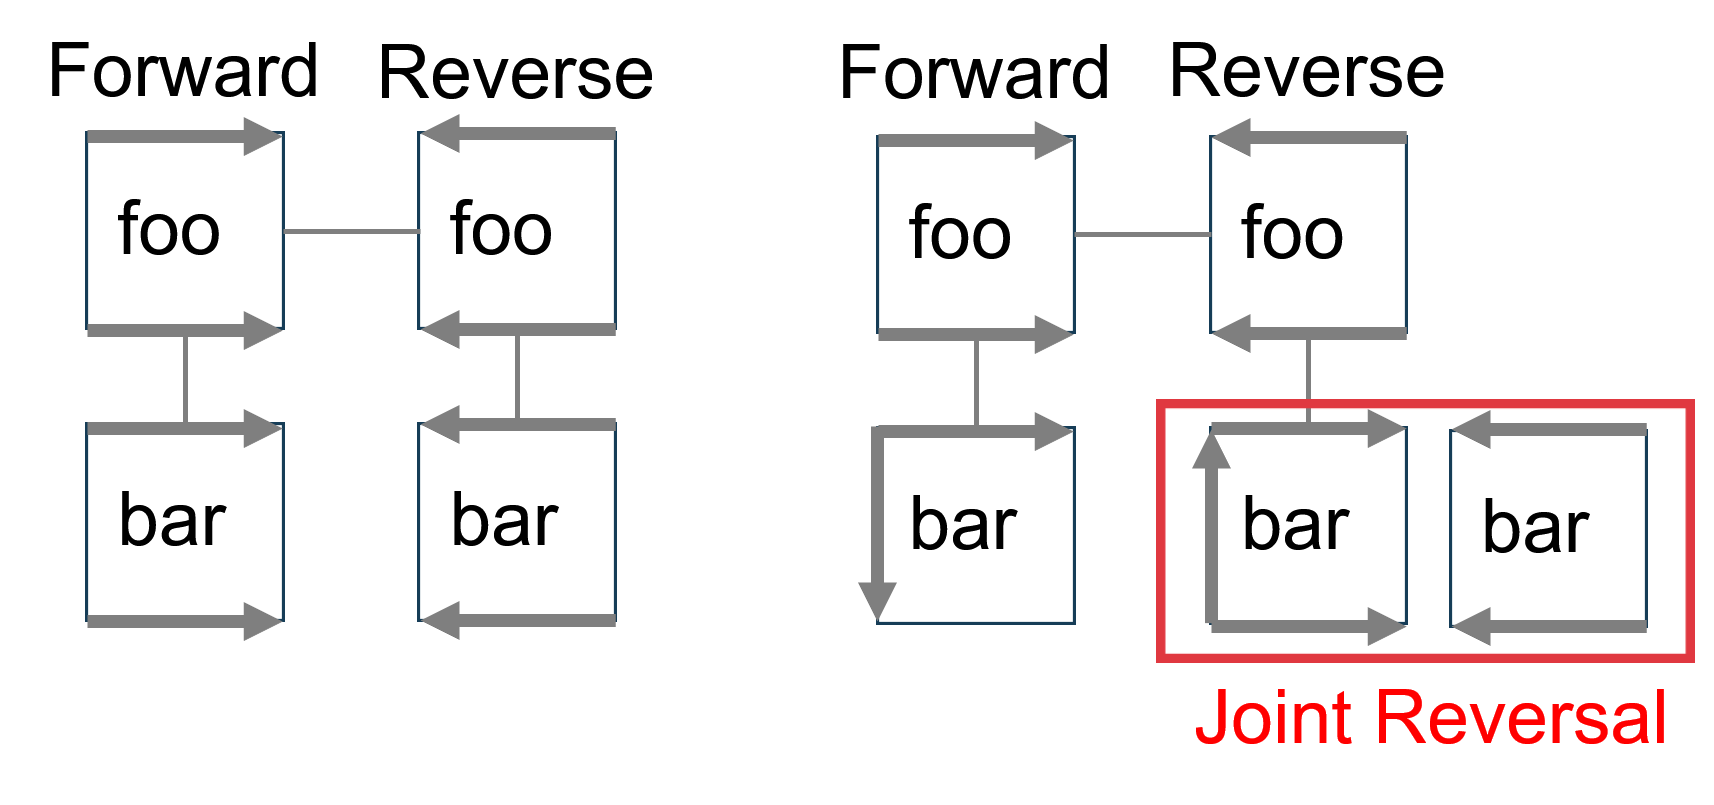
\includegraphics[width=\linewidth]{figures/joint.png}
% \caption{Reversal modes for function calls: Split reversal (left), joint reversal (right)}
% \label{fig:reversalmodes}
% \end{figure}

% % Marked as a potential for cutting text
% GPU kernels are implemented as function calls in a larger applications computer program, with the kernels being the leafs of the call tree. There are two ways of reversing a computer program for the gradient evaluation shown in \reffig{fig:reversalmodes}. {\it Split reversal} splits the entire computer program into the forward and reverse pass, where every function is first computing the primal intermediate values and storing them on a stack (double forward arrow) while restoring them (double reverse arrow) in the reverse pass. {\it Joint reversal} of a function recomputes the primal values by restoring only the inputs (up arrow) stored in the forward pass (down arrow) and then does a reverse pass in the same function call. Joint reversal trades memory storage for recomputation cost and is the obvious choice for GPU kernels with restricted memory availability; the joint reversed program uses less memory. In the following analysis we evaluate the joint reversed implementation (red) of GPU kernels.

% Rewrite of evaluation paragraph
\change{We evaluate our approach on five established GPU-based HPC proxy applications:}
\begin{itemize}
    \item CUDA-based RSBench~\cite{RSBench} and XSBench~\cite{XSBench}, two implementations of Monte Carlo neutron transport algorithms
    \item An extended version of the CUDA lattice-Boltzmann method (LBM) solver from the Parboil benchmark suite~\cite{stratton2012parboil}, with applications in computational fluid dynamics
    \item CUDA-based Livermore Unstructured Lagrangian Explicit Shock Hydrodynamics (LULESH) code~\cite{LULESH2:changes}, a proxy application for computational fluid dynamics solvers% on Exascale systems
    \item A discontinuous-Galerkin (DG) volume integral\footnote{\url{https://github.com/lcw/Heptapus.jl}}\cite{dg_wilcox} kernel as used in the pure Julia~\cite{bezanson2017julia} climate code ClimateMachine.jl\footnote{\url{https://github.com/CliMA/ClimateMachine.jl/}}~\cite{clima2017} and implemented for both CUDA and AMD GPUs
\end{itemize}


\subsection{Setup}

For each application, we time just the evaluation of the code being differentiated, excluding time taken for device memory initialization and transfer or other calling code. \change{For CUDA kernels, we explicitly increase the size of the device heap to 1 GB. RSBench, XSBench, and the CUDA.jl version of DG were evaluated on an NVIDIA 2080 Super. LBM was evaluated on an NVIDIA V100. LULESH was evaluated on an NVIDIA RTX A6000. The AMDGPU.jl version of DG was evaluated on an AMD Vega 64. Benchmarks were tested with LLVM main at commit \texttt{8dab25954b0acb53731c4aa73e9a7f4f98263030}, Julia 1.6, and Enzyme at commit \texttt{ec75831a8cb0}. The benchmark suite is available at \url{https://github.com/wsmoses/Enzyme-GPU-Tests}.}

All benchmarks were evaluated a minimum of five times, taking the geometric mean as the final result. \change{For each benchmark we evaluated the original kernel and the combined forward/reverse pass generated by Enzyme (Figure \ref{fig:app_performance}); the combined forward and reverse pass with various optimizations described in Section \ref{sec:opt} disabled (Figure \ref{fig:effect_of_optimisations}); the compile times of the benchmarks (Figure \ref{fig:comptime}); and the scalability of the gradients compared to the original code (Figures \ref{fig:relweak} and \ref{fig:probinc}).}


\begin{figure}
    \centering
    \includestandalone[width=.45\textwidth]{figures/Candlesticks}
    \caption{AD overhead of the benchmark applications, as compared with a single evaluation of the forward pass. \change{An overhead of $N$ can be read as saying that collecting the gradients of all inputs (as well as running the original code) is equivalent to running the original code $N$ times.}}
    \label{fig:app_performance}
\end{figure}

\begin{figure}
    \centering
\begin{minted}[fontsize=\small]{cuda}
void kern(float* src, float* dst) {
    streamCollide<<<...>>>(src, dst);
}

void lbm(int nTimeSteps, float* src, float* dst) {
    for (unsigned int i=0; i<nTimeSteps/2; i++) {
        kern(src, dst);
        kern(dst, src);
    }
}
\end{minted}
    \caption{\change{Simplified version of the computation within LBM. The \texttt{kern} function calls a GPU kernel that iterates the simulation one timestep forward in time, storing the result in \texttt{dst}. The \texttt{lbm} CPU function calls the GPU kernel until all iterations have completed. The iteration must happen outside the kernel to ensure that all threads from one timestep have completed prior to performing another timestep.}}
    \label{fig:lbm}
\end{figure}

\change{With the exception of the LBM benchmark (see below), modifying a benchmark to enable differentiation simply required allocating and initializing shadow arrays (to store the output gradients), and creating a kernel which calls \texttt{\_\_enzyme\_autodiff} on the kernel to be differentiated, as demonstrated in Figure \ref{fig:exdiff}.}

\change{The correctness of the generated gradients was verified by comparing with numeric differentiation. Since our benchmarks have too many parameters to use numeric differentiation effectively, only a few inputs per benchmarks were tested. }

\subsection{Benchmark Descriptions}

\paragraph{\textbf{RSBench and XSBench}}
RSBench and XSBench are U.S. Department of Energy proxy applications that represent the core computation of Monte Carlo simulations within particle transport algorithms such as in OpenMC~\cite{romano2013openmc}. The majority of the runtime of XSBench is spent in memory operations with a semi-random access pattern. By calculating neutron cross-sections with the multipole method, RSBench trades off several magnitudes of memory in exchange for a significant amount of computation to unpack the data. Together, RSBench and XSBench allow us to differentiate both compute-bound and memory-bound applications, respectively.



\begin{figure*}
    \centering
\begin{tabular}{c|c}
\textbf{(a)}&\textbf{(b)}\vspace*{-3mm}
\\
\begin{minipage}[T]{0.48\linewidth}
\begin{minted}[fontsize=\small]{cuda}
// CPU Code
void aug_kern(float* src, float *dsrc,
              float* dst, float* ddst) {
  void* tape = Allocator.allocate(...);
  aug_streamCollide<<<...>>>(src, dsrc, dst, ddst, tape);
}
void grad_kern(float* src, float *dsrc,
               float* dst, float* ddst, void* tape) {
  grad_streamCollide<<<...>>>(src, dsrc, dst, ddst, tape);
  Allocator.free(tape);
}
__attribute__((enzyme(aug_kern, grad_kern)))
void kern(float* src, float* dst);

void grad_lbm(int nTimeSteps, float* src, float* dsrc,
                              float* dst, float* ddst) {
  __enzyme_autodiff(lbm, nTimeSteps, src, dsrc, dst, ddst);
}
\end{minted}
\end{minipage}&\begin{minipage}[T]{0.48\linewidth}
\begin{minted}[fontsize=\small, escapeinside=||]{cuda}
// GPU Code
__global__
void aug_streamCollide(float* src, float* dsrc,
                       float* dst, float* ddst, void** tape) {
  size_t idx = threadIdx.x + ...;
  tape[idx] = __enzyme_augmentfwd(streamCollide, src, dsrc,
                                    dst, ddst);
}

__global__
void grad_streamCollide(float* src, float* dsrc,
                        float* dst, float* ddst, void** tape) {
  size_t idx = threadIdx.x + ...;
  __enzyme_reverse(streamCollide, src, dsrc,
                   dst, ddst, tape[idx]);
}

|\;|
\end{minted}
\end{minipage}
\end{tabular}
    \caption{\change{Differentiation of the combined CPU+GPU computation in LBM. The code in (a) represents host code, which differentiates the overall function \texttt{lbm}, defined in Figure \ref{fig:lbm}. The \texttt{kern} function is annotated with custom forward and reverse passes \texttt{aug\_kern} and \texttt{grad\_kern}. These functions allocate a tape and call the \texttt{aug\_streamCollide} and \texttt{grad\_streamCollide} kernels, which are generated by Enzyme in (b).}}
    \label{fig:lbm_ad}
\end{figure*}

\paragraph{\textbf{Lattice Boltzmann Method (LBM)}}
LBM is a particle-based fluid dynamics simulation method. It works by modeling fluid density on a lattice (grid) and in each time step performing a streaming step (allowing fluid to flow into adjacent grid cells) and a collision step (which models the interaction of fluids flowing into a particular cell from neighboring cells). This so-called stream-collide sequence is responsible for the majority of the computational cost of typical LBM solvers and is implemented in the CUDA version of Parboil LBM in a method called \texttt{performStreamCollide\_kernel}. \change{ CPU driver code calls this kernel in a loop to advance the simulation by several timesteps, as shown in Figure ~\ref{fig:lbm}. }

\change{
Unlike the other benchmarks tested, where the entire function being differentiated was on the GPU, differentiating LBM requires the differentiation of heterogeneous programs. Since LLVM does not yet support modules which contain both CPU and GPU code, we perform differentiation in two steps. First, we use Enzyme to generate an augmented forward and reverse pass for the GPU kernel. The forward pass is equivalent to the original function, saving any data that is required for the reverse pass and may be overwritten. The forward and reverse pass of the GPU kernels can then be imported into the CPU code by using Enzyme's support for custom derivatives. The heterogeneous AD setup is demonstrated in Figure ~\ref{fig:lbm_ad}. Note that while we demonstrate this shim layer for clarity, in practice this can be simplified for end users through the use of advanced compiler transformations or macros.}%
%
% There are other versions implemented e.g. for CPUs or in OpenCL, which we did not consider here.

\paragraph{\textbf{LULESH}}
LULESH~\cite{LULESH2:changes} is an unstructured explicit shock hydrodynamics solver, which was initially introduced as a proxy application for computational fluid dynamics on high-performance computing systems and has since been employed as a proxy application for complex fluid dynamics codes. % on \change{next-generation} systems. %
\change{LULESH emulates complex hydrodynamic solvers by splitting the computational domain into volumetric elements on an unstructured mesh. This allows LULESH to mimic the complex data movement characteristics of unstructured data structures.}
% AD variables were initialized through the definition in the header file and then passed down through the domain initialization into the individual kernels in the \textit{LagrangeLeapFrog} step.
All measurements were analyzed with  NVIDIA NSight Compute to discern the individual measurements of the gradient \textit{ApplyMaterialPropertiesAndUpdateVolume} kernel from the general application runtime.

\begin{figure*}
    \centering
    \includestandalone[width=\textwidth]{figures/stacked2}
    \caption{\change{Overhead of selectively disabling AD and GPU-specific optimizations described in Section \ref{sec:opt}. OOM indicates running out of memory or an indefinite runtime. Each dot represents the overhead of AD compared to the forward pass alone.}}
    \label{fig:effect_of_optimisations}
\end{figure*}

\paragraph{\textbf{Discontinuous Galerkin (DG)}}
The  discontinuous-\-Galerkin  volume integral\cite{dg_wilcox} kernel is part of a fluid dynamics simulation model. It is written in Julia, and we use \texttt{CUDA.jl}~\cite{besard2018juliagpu} and \texttt{AMDGPU.jl}~\cite{AMDGPU2021} in combination with Enzyme.jl~\cite{enzymeNeurips} to synthesize and execute the kernel and its derivative. The code features GPU-specific features, such as shared memory, and is memory bound. We modified the original code to use noncoherent memory loads in the case of \texttt{CUDA.jl} and constant memory loads in the case of \texttt{AMDGPU.jl}.

\subsection{Results}

The original Enzyme paper \cite{enzymeNeurips} demonstrated that by embedding AD within the compiler, one can perform AD after optimization which is on average $4.2\times$ faster than AD before optimization.
\change{Since prior tools perform AD at a source level, they must perform AD prior to any compiler optimizations.}
Although there exist no tools that we can compare against that perform reverse-mode AD on GPU kernels, we attempted to perform a similar ablation analysis here to see what a tool not implemented within a compiler might be able to achieve, if one were to be written. \change{ Without applying standard LLVM optimizations prior to AD, RSBench and XSBench take an indefinite amount of time to run. LULESH has an overhead of $2979.1\times$ without preprocessing optimizations. LBM is able to be differentiated without preprocessing optimizations for two iterations, but exhausts GPU memory on anything larger (scaling tests use 50-600 iterations). In order to legalize Julia code for the GPU (such as the ROCm and CUDA DG codes), it is necessary to run the LLVM optimization pipeline, along with Julia's custom optimization passes. }
We therefore conclude that the ability to run optimizations alongside AD is in fact a precondition of successful reverse-mode AD of general GPU programs.

Overall, the combined forward and gradient generated by Enzyme have a reasonable overhead when compared with that  of the forward pass (Figure~\ref{fig:app_performance}). RSBench and XSBench have a $3-4\times$ overhead due to the need to cache intermediate computations from the forward pass. Similarly, LBM must cache the current state variables every iteration leading to an overhead of $6.3\times$. The kernel evaluated in LULESH does not need to cache additional values, and as a result the \change{$2.01\times$} overhead is spent performing the corresponding gradient computations. The DG benchmark has a $5.4\times$ overhead when run on AMD, primarily from the additional computation, whereas it has a $18\times$ overhead on CUDA as it quickly exhausts the amount of available registers and the CUDA assembler decides to spill a large number of registers into global memory.

\paragraph{\textbf{AD and GPU-Specific Optimizations}}
\change{
To evaluate the effectiveness of the optimizations described in Section \ref{sec:opt}, we evaluated all benchmarks with several AD and GPU-specific optimizations being successively disabled. Not all benchmarks benefit from the same optimizations, and the order in which compiler optimizations are applied can dramatically impact performance~\cite{autophase}. For each benchmark, we visualize a path through the exponentially large optimization space that attempts to enable each optimization when it will have the largest impact on performance. The results of this analysis are shown in Figure \ref{fig:effect_of_optimisations}. An end user trying to maximize their performance wouldn't explore all optimization combinations/paths, instead simply enabling all optimizations. As disabling optimizations quickly blows up the runtime of the program, the ablation analysis of benchmarks was run at a smaller test size to ensure the computation completed in a reasonable time where necessary. 

For the ROCm DG kernel, an unrolling optimization was necessary to allow Enzyme to create the gradient without caching any additional values. Without unrolling, the GPU was unable to allocate sufficient device memory to succeed.

For the CUDA DG kernel, simply applying the standard Julia+LLVM optimization pipeline enabled the gradient to run, though at a $1378.3\times$ overhead. Running an optimization that coalesced multiple allocations into a single \texttt{malloc} call reduced this runtime to $116.6\times$. Like in the ROCm case, applying unrolling eliminates any need to cache values, reducing the overhead to $17.8\times$.

For ablation analysis, we ran the LBM kernel for 150 iterations. The use of an efficient CPU to GPU calling convention for caching values was necessary for the gradient to run on a problem of this size. Applying the improved recompute vs cache heuristic allowed Enzyme to detect that it could cache a double which representing a sum, rather than the individual of overwritten values. This analysis reduced the size of the cache from $80$ bytes per thread to $20$ bytes per thread. As a result, the AD overhead was reduced from $19.87\times$ to $8.7\times$. Finally, using a LIFO allocator rather than \texttt{cudaMalloc} to allocate cache memory brought the AD overhead down to $6.4\times$.

For ablation analysis, LULESH was run on a computational domain size of $90^{3}$. Applying just LLVM optimizations prior to AD brought the LULESH gradient overhead down to $2.4\times$ from $2979.1\times$. As the LULESH kernel was particularly branch heavy, enabling speculative execution of $\phi$ predecessors when recomputing values in the reverse pass reduced the AD overhead down to $2.01\times$.

Running RSBench on a problem size of 10,200, LLVM optimizations alone resulted in an overhead of $6374\times$. By applying additional inlining, this overhead was reduced to $9.5\times$ as LLVM could optimize between functions, enabling Enzyme to eliminate redundant values being cached, as well as use a more efficient intraprocedural caching infrastructure. Enabling the loop invariant cache and equivalent load cache optimizations reduced the overhead down to $4.7\times$.

Running XSBench on a problem size of 17,000,000 with LLVM optimizations, the overhead was $25.9\times$. Allowing Enzyme to avoid caching loop bounds when it can prove that all its instructions are inactive, drops the overhead to $16.3\times$. Performing PHI restructuring reduces the overhead to $9.5\times$. Passing the mode of simulation through a C++ template eliminates code generation of helper routines from different simulation modes and reduces the overhead to $3.2\times$. This leads to fewer branches in the forward pass and allows Enzyme to avoid analogous branches in the reverse pass.
}

% \begin{figure}
%     \centering
%     \begin{tabular}{l|r}
%          Test & Overhead \\\hline
%          Forward & 1 \\
%          AD, Optimized & 4.4 \\
%          - CacheLICM & 343.7 \\
%          - Recompute Heuristic & 1275.6 \\
%          - Inlining & 6372.2 \\
%          - PreOptimization & OOM \\
%     \end{tabular}
%     % \includestandalone[width=.45\textwidth]{figures/EffectOfOptimizations}
%     \caption{Overhead of progressively disabling AD and GPU-specific optimizations described in Section \ref{sec:opt} when evaluated on RSBench. OOM indicates that the test ran out of memory.}
%     \label{fig:effect_of_optimisations}
% \end{figure}


% \begin{figure}
%     \centering
%     \begin{tabular}{l|r}
%          Test & Overhead \\\hline
%          Forward & 1 \\
%          AD, Optimized & 3.16 \\
%          - Templating & 9.61 \\
%          - PHI Recompute & 14.47 \\
%          - Alias Analysis & 47.40 \\
%          - Recompute Heuristic & 95.75 \\
%          - PreOptimization & OOM \\
%     \end{tabular}
%     % \includestandalone[width=.45\textwidth]{figures/EffectOfOptimizations}
%     \caption{Overhead of selectively disabling AD and GPU-specific optimizations described in Section \ref{sec:opt} when evaluated on XSBench. OOM indicates that the test ran out of memory.}
%     \label{fig:effect_of_optimisations}
% \end{figure}



% \begin{figure}
%     \centering
%     \begin{tabular}{l|r}
%          Test & Overhead \\\hline
%          Forward & 1 \\
%          AD, Optimized & 6.39 \\
%          - Custom Allocator & 8.74 \\
%          - Recompute Heuristic & 19.87 \\
%          - Inline Cache ABI & OOM \\
%          - PreOptimization & OOM \\
%     \end{tabular}
%     % \includestandalone[width=.45\textwidth]{figures/EffectOfOptimizations}
%     \caption{Overhead of selectively disabling AD and GPU-specific optimizations described in Section \ref{sec:opt} when evaluated on LBM with 150 iterations. OOM indicates that the test ran out of memory.}
%     \label{fig:effect_of_optimisations}
% \end{figure}


% \begin{figure}
%     \centering
%     \begin{tabular}{l|r}
%          Test & Overhead \\\hline
%          Forward & 1 \\
%          AD, Optimized & 17.85 \\
%          - Unrolling & 116.63 \\
%          - Malloc Coalesing & 1378.32 \\
%     \end{tabular}
%     % \includestandalone[width=.45\textwidth]{figures/EffectOfOptimizations}
%     \caption{Overhead of selectively disabling AD and GPU-specific optimizations described in Section \ref{sec:opt} when evaluated on CUDA.jl DG with 20000 elements. OOM indicates that the test ran out of memory.}
%     \label{fig:effect_of_optimisations}
% \end{figure}

\begin{figure}
    \centering
    \includestandalone[width=.45\textwidth]{figures/scaling}
    \caption{Overhead of Enzyme compared with the forward pass as the problem size and number of threads increase, with constant work per thread.}
    \label{fig:relweak}
\end{figure}


\paragraph{\textbf{Scalability}}
We compare the scalability of our approach in two ways. First, we consider applications where increasing the problem size increases the number of threads, while maintaining constant work per thread. We plot the overhead as a function of problem size for DG and LULESH, XSBench, and RSBench in Figure \ref{fig:relweak}. DG on CUDA, LULESH, XSBench, and RSBench maintain a constant overhead as the problem size increases. DG on AMD's overhead increases at the start but quickly asymptotes. 
\change{
When the problem size is increased in the LBM benchmark, the amount of work and number of kernel calls increase without increasing the number of threads. As demonstrated by Figure \ref{fig:probinc}, the overhead quickly asymptotes as the additional setup required by Enzyme gets amortized across a larger number of iterations.
}

\paragraph{\textbf{LULESH Case Study}}
Automatic differentiation of LULESH's compute kernels is a prime example of the \change{importance of running optimizations prior to reverse-mode automatic differentiation on GPUs. While the generated gradient has a $2979.1 \times$ overhead without any LLVM optimizations prior to AD, this is reduced to $2.4\times$ by simply running LLVM's standard optimization pipeline. This does not require deep changes to LULESH or manual tuning. Using all the optimizations described in Section \ref{sec:opt} resulted in a reduction of the AD overhead to $\sim 2.01 \times$. Because of the effectiveness of the optimizations and low overhead, we looked at the memory access patterns in depth to understand the impact Enzyme and its optimizations had on the memory system of the GPU.}

In Figure~\ref{fig:memory_hierarchy}, we analyze the memory characteristics of the \textit{ApplyMaterialPropertiesAndUpdateVolume} kernel, using NVIDIA's NSight-Compute analyzer. We use the memory workload analysis as a guide \change{to evaluate the performance of the synthesized gradient kernel and judge whether there are potentially missed optimizations, or common access patterns within the gradient kernel}. For this kernel, the profile shows that there is an $\sim 50\%$ increase in memory traffic when performing gradient calculations. If excessive caching or register spilling occurred, we would \change{have seen} an increase in \emph{Local} memory traffic. This performance report is typical of an efficient gradient kernel, which is reflected in the low AD overhead of $2.01\times$. % (see Figure~\ref{fig:app_performance}).

\begin{figure}
    \centering
    \includestandalone[width=.45\textwidth]{figures/scaling2}
    \caption{Overhead of Enzyme compared with the forward pass where work is increased while maintaining a constant number of threads.}
    \label{fig:probinc}
\end{figure}


\paragraph{\textbf{Discontinuous Galerkin (DG) Case Study}}
\label{par:dg}
We evaluated the DG kernel on both AMD and NVIDIA GPUs. The NVIDIA variant shows \change{an} overhead of $18\times$ versus an overhead of $5.4\times$ for the AMD variant. Performance analysis of the NVIDIA implementation unveiled two bottlenecks in the gradient kernel. The first bottleneck was caused by a large number of values reused from the forward pass. This created excessive register spilling and correspondingly increased global memory traffic. Second, some atomic increment operations on shared memory were heavily contended. Surprisingly, the AMD implementation performs much better. \change{We hypothesize that AMD is faster because the AMDGPU LLVM backend directly optimizes for the target architecture and can perform optimizations such as target register allocation.} In contrast, the NVIDIA LLVM backend targets NVIDIA's virtual instruction set architecture NVPTX and leaves register allocation to \texttt{ptxas}.

% Note, for final version we should have the parallelism turned off experiment here

Enzyme allows  the user to specify whether the gradient should be calculated with respect to an argument. We used the DG kernel to verify that applying Enzyme with all arguments set to be constant (not differentiated), would not incur any overhead.


\begin{figure}
    \centering
    \rotatebox{-90}{\resizebox{0.6\textwidth}{!}{\import{figures}{revised_memory_hierarchy3.pdf_tex}}}
    \caption{Memory workload analysis for LULESH \change{at} size $135^{3}$ \change{comparing the original code (Fwd) to the gradient (AD)}. %
    %Of note is the increase in instructions that perform a 
    %\emph{global} load and store, by \change{$50\%$}, resulting in an additional \change{$\sim 27.5\%$} memory traffic increase to the device memory.
    }
    \label{fig:memory_hierarchy}
\end{figure}

\paragraph{\textbf{Compile Time}}
\label{par:compile}
\change{
We compare the time spent to compile kernels with and without the gradient generated by Enzyme. In practice, when running large simulations the compile time is negligible compared with the runtime. Nevertheless, it is useful to verify that also compiling the derivatives does not substantially change the program's overall compile time. For the four C/C++ benchmarks (LBM, LULESH, RSBench, and XSBench), we measured just the compile time of the file that contained the kernel being differentiated. This is then compared with compiling the same source file, but also generating all the requisite derivative information. This involves creating additional functions, running a second round of optimizations, and running the backend code generator for the additional kernel(s). For codes that just compile the combined forward and reverse passes (LULESH, RSBench, and XSBench), we would expect a $\sim 3\times$ overhead as in addition to the original kernel, there is now a second kernel which is twice the size (containing the forward and reverse pass). For codes in which a forward and reverse pass are requested separately, we would expect a $\sim 4\times$ overhead to account for the additional augmented forward pass, and the split reverse pass (which contains its own forward and reverse pass). These compile times are all within expectation.


The two Julia codes must be analyzed separately. As Julia is a JIT, Enzyme.jl works by running its own additional compilation within Julia's runtime and performing foreign function calls into Enzyme loaded as a dynamic library As a result, a direct comparison is not meaningful. Nevertheless we demonstrate that the ``forward'' time, taken to compile the original kernel, is comparable with the ``AD'' time to perform a foreign function call to \texttt{libEnzyme.so}, which generates the derivative runtime function.
% Nevertheless, it is useful to verify that also compiling the derivatives does not dramatically change the compile time of the program. 
}
\section{Conclusion}
\label{sec:conclusion}

By extending Enzyme, an AD tool for LLVM, we have created the first AD tool capable of generating gradients of GPU kernels without rewriting entire applications with a differentiable DSL. Reverse-mode differentiation of GPU kernels adds several challenges including potential data races caused by the GPU's parallelism and the GPU's complex performance characteristics. We demonstrate an algorithm for differentiating GPU-based parallel control flow and other intrinsics that ensures the correctness of the resultant gradients. To maximize performance of the generated gradients, we introduce several novel AD and GPU-specific optimizations. Through various ablation analyses, we show how without these optimizations reverse-mode GPU AD is intractable in practice.  We demonstrate reasonable performance and scalability on several applications relevant to the HPC community.


\begin{figure}
    \centering
    \begin{tabular}{l|r|r|r}
         Test & Forward & AD & Overhead\\\hline
         LBM & 1.54 & 5.65 & 4.32$\times$\\
         LULESH & 8.34 & 23.82 & 2.86$\times$\\
         RSBench & 14.99 & 33.29 & 2.22$\times$\\
         XSBench & 15.9 & 23.5 & 1.48$\times$\\
         \hline
         Julia DG CUDA & 0.50 & 3.41 & 6.82$\times$\\
         Julia DG AMD & 1.12 & 2.56 & 2.29$\times$\\
    \end{tabular}
    \caption{\change{Compile time in seconds of the source file with and without derivatives.}}
    \label{fig:comptime}
\end{figure}

%\subsection{Future work}
\change{There exist} several avenues for future work. Many of the optimizations described in Section~\ref{sec:opt}, especially those involving caching, could make better use of shared memory, when available. For example, with rare exception, Enzyme currently maintains the GPU schedule described in the forward pass for use in the reverse. One could imagine allowing Enzyme to reschedule a kernel in such a way that minimizes potential races and therefore allows better performance. Moreover, Enzyme currently identifies constant shared-memory indices as the only scenarios where it can perform a reduction rather than falling back to an atomic increment. Extending Enzyme to more aggressively identify locations where it can perform a reduction rather than atomics can result in additional performance boosts, especially in kernels that, like the DG kernel, make heavy use of shared memory (see Section~\ref{par:dg}). Extending Enzyme to support Forward and Mixed-Mode \cite{besard2018juliagpu} AD may provide potential performance boosts by allowing Enzyme to choose the differentiation algorithm expected to perform fastest for a particular workload. Moreover, support for parallelism demonstrated here in the context of GPUs can be extended to support both CPU parallelism and distributed frameworks such as MPI to allow Enzyme to efficiently differentiate a wider variety of HPC applications.

\begin{acks}
{
%\footnotesize
%\fontsize{8.5}{9.5} \selectfont
\small
Many thanks to Paul Hovland (ANL) for plenty of thoughtful suggestions on automatic differentiation.
The authors would like to thank Lilly Chin (MIT) for their help in performing numerous hardware upgrades, without which this work would not have been possible.

% The information, data, or work presented herein was funded
% in part by NSF Grant OAC-1835443 and by DARPA under agreement number HR0011-20-9-0016 (PaPPa). 

% This material is based upon work supported by the Department of Energy, National Nuclear Security Administration under Award Number DE-NA0003965.

William S. Moses was supported in part by a DOE Computational Sciences Graduate Fellowship
DE-SC0019323. Valentin Churavy was supported in part by the Defense Advanced Research
Projects Agency (DARPA) under Agreement No. HR0011-20-9-0016, and in part by NSF Grant
OAC-1835443. Ludger Paehler was supported in part by the German Research Council (DFG) under grant agreement No. 326472365. This research was supported in part by Los Alamos National Laboratories grant
531711; in part by the Applied Mathematics activity within the U.S. Department of Energy, Office of Science, Advanced Scientific Computing Research Program, under contract number DE-AC02-06CH11357; in part by the Exascale Computing Project (17-SC-20-SC), a collaborative effort of two U.S. Department of Energy organizations (Office of Science and the National Nuclear Security Administration) responsible for the planning and preparation of a capable exascale ecosystem, including software,applications, hardware, advanced system engineering, and early testbed platforms, in support of the nation's exascale computing imperative; and in part by the United States Air Force Research Laboratory and the United States Air Force Artificial Intelligence Accelerator and was accomplished under Cooperative Agreement Number FA8750-19-2-1000. The views and conclusions contained in this document are those of the authors and should not be interpreted as representing the official policies, either expressed or implied, of the United States Air Force or the U.S. Government. The U.S. Government is authorized to reproduce and distribute reprints for Government purposes notwithstanding any copyright notation herein. We gratefully acknowledge the computing resources provided and operated by the Joint Laboratory for System Evaluation (JLSE) at Argonne National Laboratory.


% Disclaimer: "This report was prepared as an account of work sponsored by an agency of the United States Government. Neither the United States Government nor any agency thereof, nor any of their employees, makes any warranty, express or implied, or assumes any legal liability or responsibility for the accuracy, completeness, or usefulness of any information, apparatus, product, or process disclosed, or represents that its use would not infringe privately owned rights. Reference herein to any specific commercial product, process, or service by trade name, trademark, manufacturer, or otherwise does not necessarily constitute or imply its endorsement, recommendation, or favoring by the United States Government or any agency thereof. The views and opinions of authors expressed herein do not necessarily state or reflect those of the United States Government or any agency thereof."
}
\end{acks}


%%
%% The next two lines define the bibliography style to be used, and
%% the bibliography file.
\bibliographystyle{ACM-Reference-Format}
\bibliography{references}
\clearpage
\appendix
\section{Artifact Description/Artifact Evaluation}
%\documentclass[sigconf,review,anonymous]{acmart}

%\begin{document}

Our paper explored how reverse-mode automatic differentiation could be performed on existing GPU kernels by extending the Enzyme automatic differentiation engine for LLVM. The paper demonstrates how various novel optimization passes and differentiation rules for GPU instructions allow for correct and efficient evaluations of the gradient.

The paper evaluated 6 benchmarks: XSBench (CUDA), RSBench (CUDA), Parboil LBM (CUDA), LULESH (CUDA), DG (CUDA), DG (AMD). Of these benchmarks, the AMD and CUDA DG codes are Julia-based where as the remainder are C++/CUDA. All benchmarks are available on Github \url{https://github.com/wsmoses/Enzyme-GPU-Tests} at commit \verb|d4daa0cd5931494bc4dfbfffc7874c3b00b1e3a4| with a DOI of \verb|10.5281/zenodo.5147573|. Evaluation of these benchmarks allowed the paper to demonstrate the efficiency of the generated gradients in comparison to the original code, the impact of the novel optimizations, the scalability of the generated gradients, and the correctness of the tool.

To run the benchmarks used in the paper, we first need to build the LLVM compiler toolchain before we can subsequently link the compiler plugin of Enzyme against our built LLVM version. For our compiler toolchain we used LLVM 13 (main) at commit \verb|8dab25954b0acb53731c4aa73e9a7f4f98263030|. To install LLVM, please follow the following steps:

\begin{minted}[fontsize=\small, escapeinside=||]{bash}
$ cd ~
$ git clone https://github.com/llvm/llvm-project
$ cd llvm-project
$ git checkout 8dab25954b0acb53731c4aa73e9a7f4f98263030
$ mkdir build && cd build
$ cmake ../llvm -DLLVM_ENABLE_PROJECTS="clang" \
-DLLVM_TARGETS_TO_BUILD="X86;NVPTX" \
-DCMAKE_BUILD_TYPE=Release -G Ninja
$ ninja # This may take a while
# clang is now be available
# in ~/llvm-project/build/bin/clang
\end{minted}

We now must build an Enzyme based off of our chosen LLVM version. We use Enzyme at commit \verb|ec75831a8cb0170090c36|.

\begin{minted}[fontsize=\small, escapeinside=||]{bash}
$ cd ~
$ git clone https://github.com/wsmoses/Enzyme
$ cd Enzyme/enzyme
$ git checkout ec75831a8cb0170090c366f8da6e3b2b8
$ mkdir build && cd build
$ cmake ../enzyme -DLLVM_DIR=/path/to/llvm/build \
-DCMAKE_BUILD_TYPE=Release -G Ninja
$ ninja
# ClangEnzyme-13.so will now be available in 
~/Enzyme/enzyme/build/Enzyme/ClangEnzyme-13.so
\end{minted}

Some of the C++ benchmarks require a custom CUDA libdevice (the implementation of various CUDA intrinsics). This is to remedy an issue within LLVM that prevents common math functions from being identified as LLVM intrinsics (this is being worked on upstream). For the default CUDA installation, libdevice can be found at \verb|/usr/local/cuda/nvvm/libdevice.10.bc|. The following code snippet describes how to replace a libdevice file, assuming you are using CUDA 11.2. The instructions are similar for a different CUDA installation, with the path changed accordingly. Note that you may need to be root to perform the change, and that you should always make a backup of your previous libdevice.

\begin{minted}[fontsize=\small, escapeinside=||]{bash}
# Save a copy of your current libdevice
$ sudo cp /usr/local/cuda-11.2/nvvm/libdevice/libdevice.10.bc\
 /usr/local/cuda-11.2/nvvm/libdevice/libdevice.10.bc.old
$ sudo cp /path/to/new/libdevice.10.bc\
 /usr/local/cuda-11.2/nvvm/libdevice/libdevice.10.bc
\end{minted}

We have created Python3 scripts to ease setting up and running our experiments. They will attempt to deduce appropriate paths given the following environmental variables. In the event that there is an issue, you likely may need to change \verb|bench.py| or the \verb|Makefile| for the test as appropriate. All of the \verb|bench.py| benchmarking scripts follow the same structure.

\begin{minted}[fontsize=\small, escapeinside=||]{bash}
# The index of the CUDA GPU desired
$ export DEVICE=1
# The path to the CUDA installation
$ export CUDA_PATH=/usr/local/cuda-11.2
# The path to the Clang++ binary we built above
$ export CLANG_PATH=/path/to/llvm/build/bin/clang++
# The path to the Enzyme plugin we built above
$ export ENZYME_PATH=\
/path/to/Enzyme/enzyme/build/Enzyme/ClangEnzyme-13.so
\end{minted}

Let's now clone the benchmark suite.

\begin{minted}[fontsize=\small, escapeinside=||]{bash}
$ git clone https://github.com/wsmoses/Enzyme-GPU-Tests
\end{minted}

The benchmark suite folder breaks down into the following structure:

\begin{itemize}
    \item DG, a Discontinuous Galerkin benchmark (CUDA \& ROCm in Julia)
    \item LBM, a Lattice Boltzmann benchmark (CUDA in C++)
    \item LULESH, a Lagrangian Hydrodynamics benchmark (CUDA in C++)
    \item RSBench, a Monte Carlo Particle Transport benchmark (CUDA in C++)
    \item XSBench, a Monte Carlo Particle Transport benchmark (CUDA in C++)
\end{itemize}

We can now enter one of the 4 C++ test directories (XSBench, RSBench, LBM, LULESH) and run the corresponding benchmark.

\begin{minted}[fontsize=\small, escapeinside=||]{bash}
$ cd Enzyme-GPU-Tests/LBM
$ python3 bench.py
# output of benchmark times printed out here
\end{minted}

The \verb|bench.py| script will run first an ablation analysis that enables or disables differentiation, along with several optimizations. The result of these tests will be the execution time of the gradient and/or original kernel. The script will then run by scaling tests for both the gradient and original kernel by evaluating on increasing problem sizes. Some benchmarks (XSBench, LBM, LULESH, DG (CUDA)) will end by printing out the derivative as computed by both numeric differentiation and Enzyme. These will include "\verb|VERIFY=yes|" as part of the run line. All other run lines will contain the execution time of that benchmark. Be aware that LULESH's ablation analysis includes benchmarks configurations, which do not perform compiler optimizations and are hence significantly slower than the other benchmarks.

XSBench and RSBench require the libdevice found in Enzyme-GPU-Tests/libdevice1, and were run using CUDA 11.2 on an NVIDIA 2080 Super.

LBM uses the packaged libdevice from NVIDIA and was run using CUDA 11.3 on an NVIDIA V100.

LULESH uses the libdevice found in Enzyme-GPU-Tests/libdevice2 and was run using CUDA 11.2 on an NVIDIA A6000. The LULESH benchmark suite furthermore relies on NVIDIA's N-Sight compute utility (NCU). NCU has known issues with access to the GPU Performance counters, which you will need to benchmark the gradient kernel of LULESH. If you should run into this issue please have a look at the following documentation to remedy it \url{https://developer.nvidia.com/nvidia-development-tools-solutions-err-nvgpuctrperm-nvprof}.

Odd performance results or a compiler error is a potential indicator of using an incorrect libdevice.

For example, when compiling one of the ablation tests of RSBench without the correct libdevice, one may see the following error when running \verb|bench.py|:
\begin{verbatim}
cannot handle (augmented) unknown intrinsic
  %5 = tail call i32 @llvm.nvvm.d2i.hi(double %0) #21
error in backend: (augmented) unknown intrinsic
clang-13: error
\end{verbatim}

The two DG tests were run using Julia 1.6. Julia at this version must be found in your path before being able to run the Julia tests. To obtain a working Julia installation see \url{https://julialang.org/downloads/} and follow the provided installation instructions.

DG (CUDA) was run with the libdevice found in Enzyme-GPU-Tests/libdevice1 on CUDA 11.2 by an NVIDIA 2080 Super.

DG (AMD) was run on an AMD Vega 64.

We have provided a similar \verb|bench.py| script for DG. While printed in a different format (CSV-style), it contains the same information about runtimes for both ablation and scaling as the C++ CUDA tests (DG AMD does not have an ablation analysis as it does not run without all optimizations applied).


\begin{minted}[fontsize=\small, escapeinside=||]{bash}
$ cd Enzyme-GPU-Tests/DG/cuda
$ python3 bench.py
\end{minted}

Note that the numeric verification may come earlier in the script's output, and should look something like this:
\begin{verbatim}
# Enzyme derivative as the first element of tuple
# followed by numeric approximation on the right
(dQ.dval[1], (o2 - o1) / 0.0001) =\ 
(-1.105959f0, [-1.10626220703125])
\end{verbatim}

The forward pass alone in the CSV-style output are denoted as the "primal" rows, whereas the derivative runtimes are marked as "all\_dub".

The DG tests may require additional setup. For example, you see an output like below (note that this may also occur if you try to run DG (AMD) on a system without the relevant AMD libraries available).
\begin{verbatim}
Warning: HSA runtime has not been built,\
runtime functionality will be unavailable.
Please run Pkg.build("AMDGPU") and reload AMDGPU.
\end{verbatim}

You may then need to explicitly run various setup routines within Julia's package manager. To fix the Julia setup for the test, perform the following to enter an interactive shell.

\begin{minted}[fontsize=\small, escapeinside=||]{bash}
$ cd Enzyme-GPU-Tests/DG/rocm
$ julia --project=.
julia> using Pkg; Pkg.build("AMDGPU")
\end{minted}


%\end{document}
\end{document}
\endinput
%%
%% End of file `sample-acmtog.tex'.
